% Note that if you want something in single space you can go back and
% forth between single space and normal space by the use of \ssp and
% \nsp.  If you want doublespacing you can use \dsp.  \nsp is normally
% 1.5 spacing unless you use the doublespace option (or savepaper
% option)
%
%(FORMAT) Usually you *don't* want to mess with the spacing for your
%(FORMAT) final version.  If you think/know that the thesis template
%(FORMAT) and/or thesis style file is incorrect/incomplete, PLEASE
%(FORMAT) contact the maintainer.  THANK YOU!!!

\chapter{Motifs}
\label{section:Motifs}

Motifs are the primary object of interest as a way of characterizing the local structure of a
network. The dynamic motif count indicates the network and the communities within are evolving according to certain rules.
In the context of static networks, the frequency of motifs 
has been shown to highlight system properties in networks \cite{bioAlbert} \cite{biomotif}.

Motifs are the fundamental components of complex systems.
The topological structure of complex networks
is tied to the frequency and distribution of motifs. Initially, the counting of 
these motifs was treated as a static problem where the frequencies of motifs affect functions on networks \cite{motifdiscovery}.
As the significance of motifs has become more apparent, authors have begun examining the emergence of motifs 
via temporal edges \cite{temporalmotifs}. Our motif counts will
act as a vector of features characterizing the network at each point in time. Before we
examine our specific motifs, we must first define common objects of graph theory such as cycles, paths, and stars
which will aid us in understanding the motifs we would like to examine.

\section{Graph Theory}

In the pursuit of counting our particular motifs, we require some
ideas from graph theory. We will count three-cycles, four-cycles, and five-cycles
as motifs, but we also require the non-simple cycle motifs.
Much of the literature on motifs focuses on directed triangle motifs  \cite{Milo824} \cite{temporalmotifs} \cite{Interactome}, but 
 the motifs can take on other shapes. The motifs in this thesis are undirected but more varied in edge and node count.
 Graphs are the common language of motifs. We define a graph $G$ by the following definition.

\begin{dfn}
    Let $G = (V,E)$ be a graph with $V$ being a set of vertices (or nodes), 
and $E$, a set of edges. If $v$ is a vertex of $G$ we write $v \in V(G)$. 
If $u,v \in V(G)$ and there is an edge between them we 
write $\{u,v\} \in E(G)$
\end{dfn}

Graphs may be directed or undirected. For directed graphs $\{u,v\} \in E(G)$
is taken to mean there exists an edge from $u$ to $v$ in $G$. Undirected implies the 
edge between $u$ and $v$ has no notion of direction.

\begin{dfn}
    The adjacency matrix $A$ for any graph $G$ with $n=|V|$ vertices is a matrix of size
    $n \times n$. The element $a_{i,j}$ is defined to be
    $$
    a_{i,j} = 
    \begin{cases}
        1 \quad e_{i,j} \in E(G)\\
        0 \quad e_{i,j} \not \in E(G)\\
    \end{cases}
    $$
    \label{def:adjmat}
\end{dfn}

\noindent The adjacency matrix is critical to all of our calculations to come. It renders
any graph amenable to the tools of linear algebra.

\begin{dfn}
\label{def:homomorphism}
We call $f: G \rightarrow H$ a homomorphism,
if $f$ maps endpoints in $G=(V(G),E(G))$ to endpoints in $H=(V(H),E(H))$.
i.e. $ \forall u,v \in V(G) \quad \{u,v\} \in E(G) \Rightarrow \{f(u),
f(v)\} \in E(H)$.
\end{dfn}


\noindent  For example, in Figure~\ref{fig:homomorphism} we can define a mapping $f$ such that:

\begin{align*}
    &f(0) = A\\
    &f(1) = A\\
    &f(2) = B\\
    &f(3) = C\\ 
\end{align*}

\noindent Thus $f$ is a homomorphism by Definition~\ref{def:homomorphism}. 
We now define the isomorphism and automorphism.


\begin{figure}[h!]
    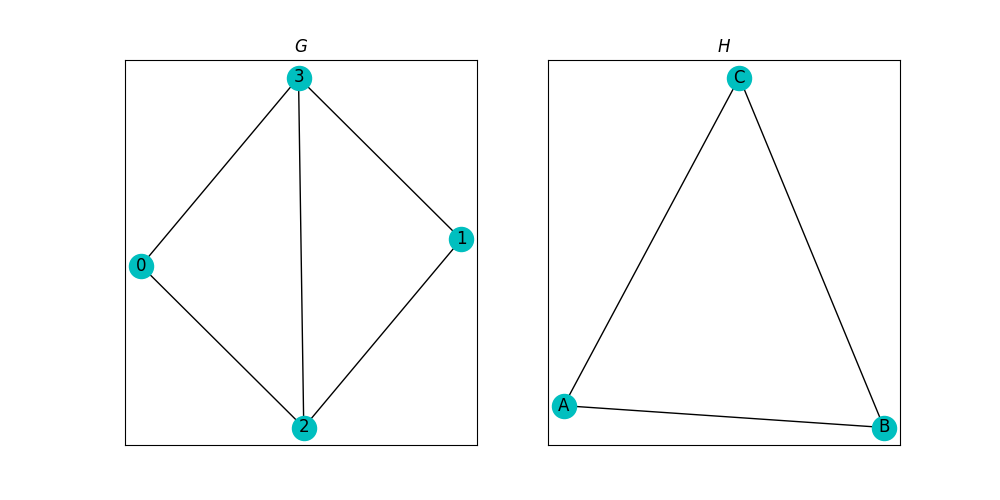
\includegraphics[width=10cm]{Images/graph_homomorphism.png}
    \centering
    \caption{A homomorphism from G to H.}
    \label{fig:homomorphism}
\end{figure}


\begin{dfn}
    We call $f: G \rightarrow H$ an isomorphism
 if $f$ is a homomorphism and is bijective.
\end{dfn}

\noindent We can define an isomorphism $f$ for between $G$ and $H$ in the figure ~\ref{fig:isomorphism} such that:

\begin{align*}
    &g(0) = B\\
    &g(1) = A\\
    &g(2) = C\\
    &g(3) = D\\ 
\end{align*}

\begin{dfn}
    An automorphism is an isomorphism between a graph $G$ and itself. The automorphism 
    is edge-preserving, $\{u,v\} \in G \implies \{f(v),f(u)\} \in G$.
\end{dfn}

\begin{figure}[h!]
    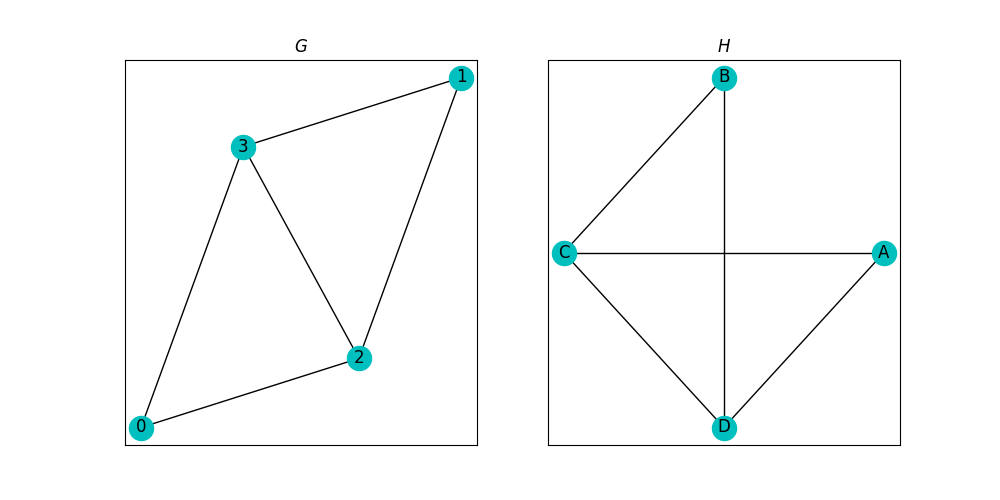
\includegraphics[width=12cm]{Images/graph_isomoprhism.png}
    \centering
    \caption{An isomorphism between $G$ and $H$.}
    \label{fig:isomorphism}
\end{figure}

Automorphisms represent the symmetries of a graph. For instance, a $C_3$ with vertices $\{A, B, C\}$
and the set of undirected edges $\{A,B\},\{B,C\},\{C,A\},$ has six possible automorphisms - three from rotation 
and three from reflection of the graph. When counting motifs on graphs, the algorithms only count up to symmetry.
For instance, where we find an induced subgraph isomorphic to $C_3$ we count the subgraph as a
 single appearance of the triangle motif. 


\begin{dfn}
    Let $G=(V,E)$ be a graph. We call $G'=(V',E')$ a subgraph, denoted $G' \subset G$, if
     $V' \subseteq V \land E' \subseteq E \cap (V' \times V')$. Furthermore we call $G'$
     an induced subgraph of $G$ if $\forall u,v \in V$ we have $\{u,v\} \in E \iff \{u,v\} \in E'$.
\end{dfn}

\noindent Induced subgraphs are vital to our understanding of how motifs interact as we add edges or nodes
to a given graph. In Figure~\ref{fig:subgraph}, $G$ has a subgraph which does not include the edge $\{1,2\}$. If
the edge is included in the set then we have an induced subgraph of $G$.

\begin{figure}[h!]
    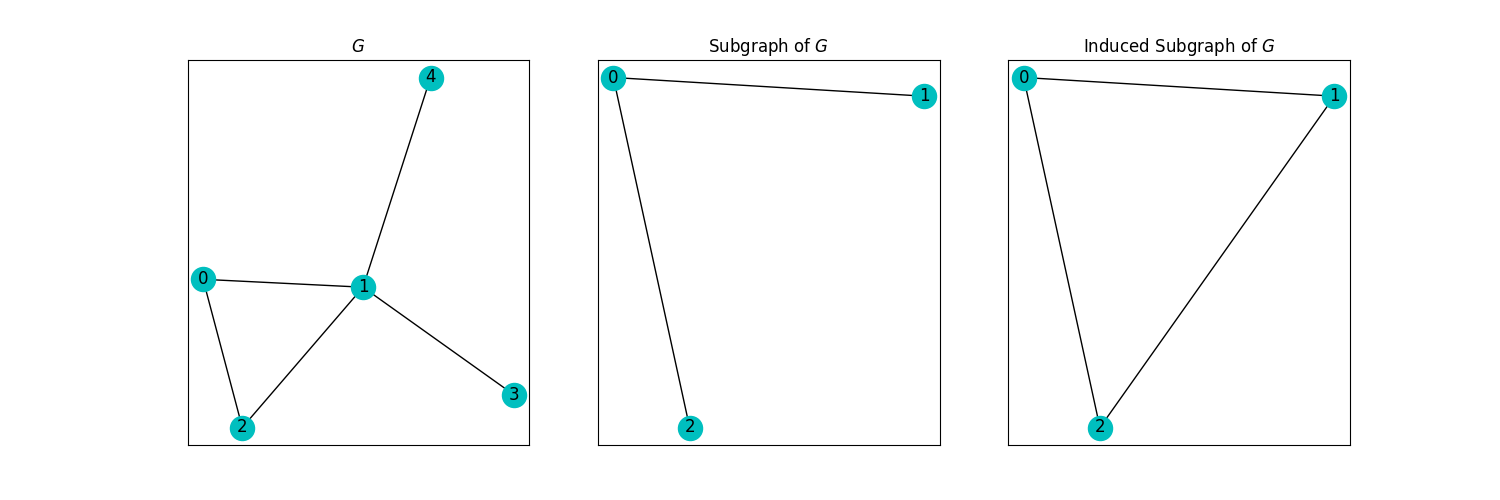
\includegraphics[width=0.8\linewidth]{Images/subgraph.png}
    \centering
    \caption{Example of subgraphs and induced subgraphs on $G$.\label{fig:subgraph}}
\end{figure}

\begin{dfn}
    Let $G'' \subset G$ and furthermore let there exist an isomorphism between $G''$ and $G'$. We call
    $G''$ an appearance of $G'$. Provided the number of appearances of $G'$ is greater than some $N$ we call $G'$
    a motif or pattern. The count of $G'$ refers to the number of appearances of $G'$ in $G$. 
\end{dfn}

\begin{dfn}
    A walk $W = \{v_0, e_1, v_1, \dots v_n\}$ is a sequence of edges and vertices of $G$ such that
    for $0 \leq k \leq n-1$ the edge $e_i = \{v_k, v_k+1\}$.
\end{dfn}

\begin{dfn}
    A cycle $Cn$ is a walk of $n$ vertices, whose first and last vertex are the same.
\end{dfn}

Cycles are often also referred to by the geometric objects they resemble. A three-cycle is a triangle and a four-cycle is a square.
The three-cycle, four-cycle, and five-cycle will feature as motifs in our feature vectors. A five-cycle is shown in 
Figure~\ref{fig:cycle}. 

\begin{figure}[h!]
    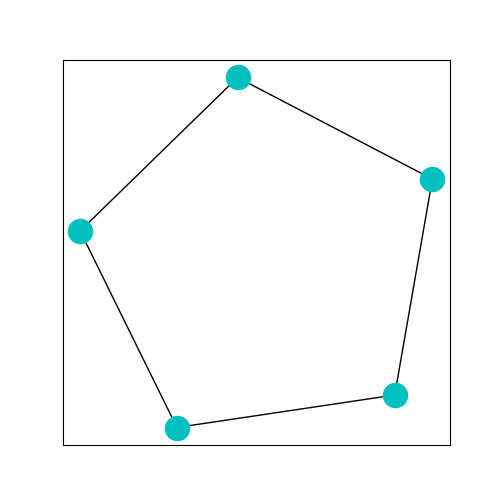
\includegraphics[width=8cm]{Images/Cycle.png}
    \centering
    \caption{A simple cycle of length five, denoted $C_{5}$.\label{fig:cycle}}
\end{figure}

\begin{dfn}
    A bipartite graph is a graph whose nodes may be separated into two disjoint sets $U$ and $V$
    such that there exists an edge between all vertices in $U$ and all vertices in $V$.
\end{dfn}

The $C_{3}$ and $C_{4}$ motif counts are themselves a measurement of node clustering in the graph. The
global clustering coefficient defined in Chapter one explicitly requires the $C_{3}$ count in its 
calculation. We count a single bipartite motif: the star $S_3$.
An example of $S_4$ can be found in Figure~\ref{fig:star}.

\begin{dfn}
    A star $S_n$ denotes the complete bipartite graph $K_{1,n}$. In other words, 
    a tree with one internal node, but $n$ branches.
\end{dfn}

\FloatBarrier

\begin{figure}[h!]
    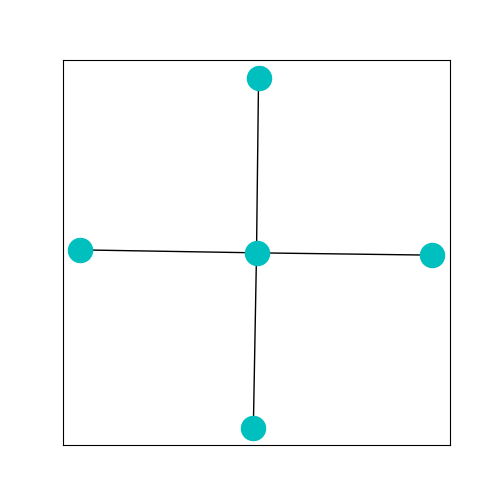
\includegraphics[width=8cm]{Images/Star.png}
    \centering
    \caption{The star $S_4$. \label{fig:star}}
\end{figure}

\newpage

\section{Non-Simple Cycle Motifs}
\label{section:Non-simple Motifs}
We wish to consider motifs that we refer to as $H_{3}$ up to $H_{13}$.
These motifs, and their enumerations, are described in Alon et al.\cite{alon} In Figure~\ref{fig:motifs1}
are the graphs of all eleven non-simple cycle motifs.

\begin{dfn}
    Let $f$ be a homomorphism between graphs $G$ and $H$. We say that $H$ is a
    homomorphic image of $G$ provided $f$ is surjective.
\end{dfn}

\begin{dfn}
    A graph $H = (V(H), E(H))$ is said to be k-cyclic, for $k > 3$, if it is a
homomorphic image of the cycle $C_k$. The number of different homomorphisms from $C_k$
to $H$ is denoted by $C_k(H)$.  $H$ is $k$-cyclic if and only if $C_k(H) > 0$.
\end{dfn}

These motifs are non-simple cycles. For the motifs in Figure ~\ref{fig:motifs1}, we can classify them to their homomorphic images. $H_{3}$, $H_{4}$, $H_{6}$, $H_{9}$, and $H_{11}$ are all six-cyclic. $H_{5}$
is the only five-cyclic graph. However $H_{5}$, $H_{6}$, $H_{7}$, $H_{8}$, $H_{10}$, $H_{12}$, and $H_{13}$ are 
all seven-cyclic.

\begin{figure}[ht!]
    \frame{\includegraphics[width=0.6\linewidth]{Images/mega_motif.png}}
    \centering
    \caption{The eleven non-simple motifs. This set is comprised
    of structurally different graphs. For instance, there is a three-walk ($H_{3}$), a star $S_3$ ($H_{4}$), the star $S_3$ with two vertices
    attached ($H_{5}$), and an $S_3$ with two edges added. The motif counts differ wildly depending on a graph's attachment mechanism(s). \label{fig:motifs1}}
\end{figure}

% \begin{figure}[h!]
%     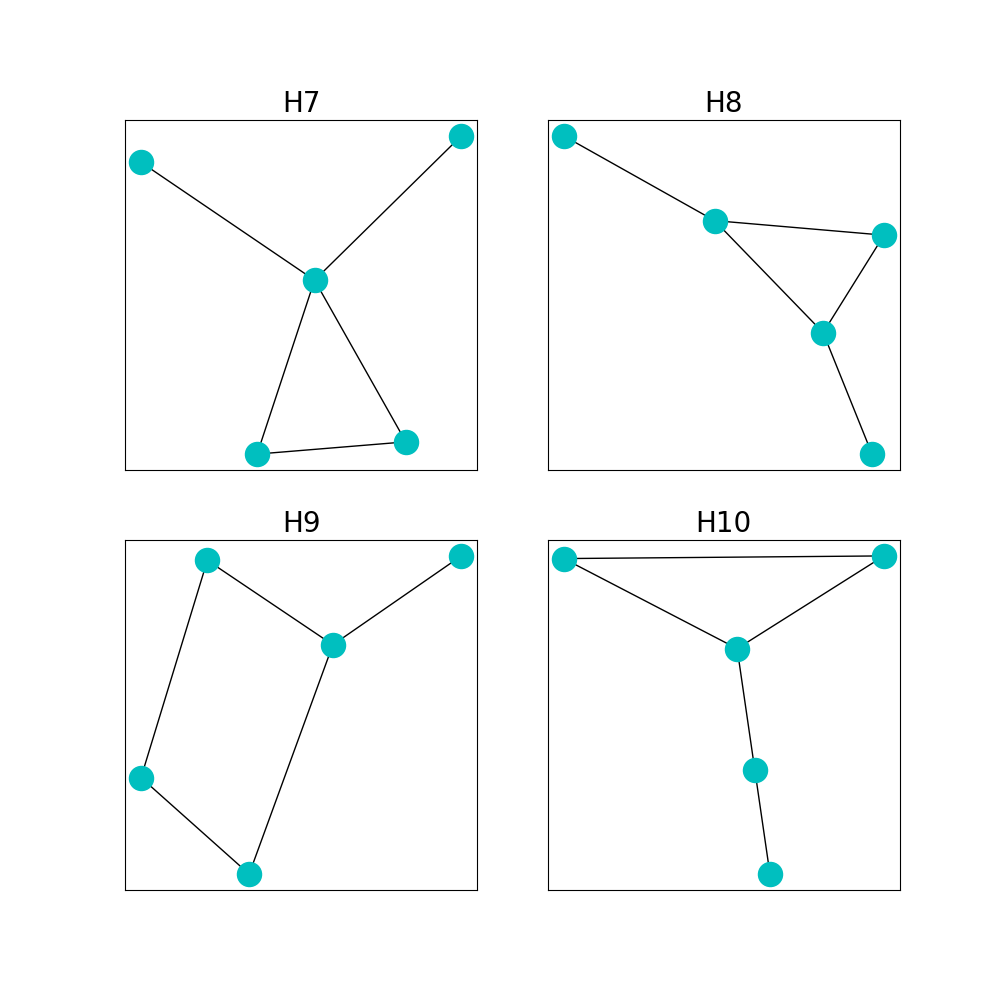
\includegraphics[width=9cm]{Images/motif_set_two.png}
%     \centering
%     \caption{Four more non-simple motifs}
%     \label{fig:motifs2}
% \end{figure}

% \begin{figure}
%     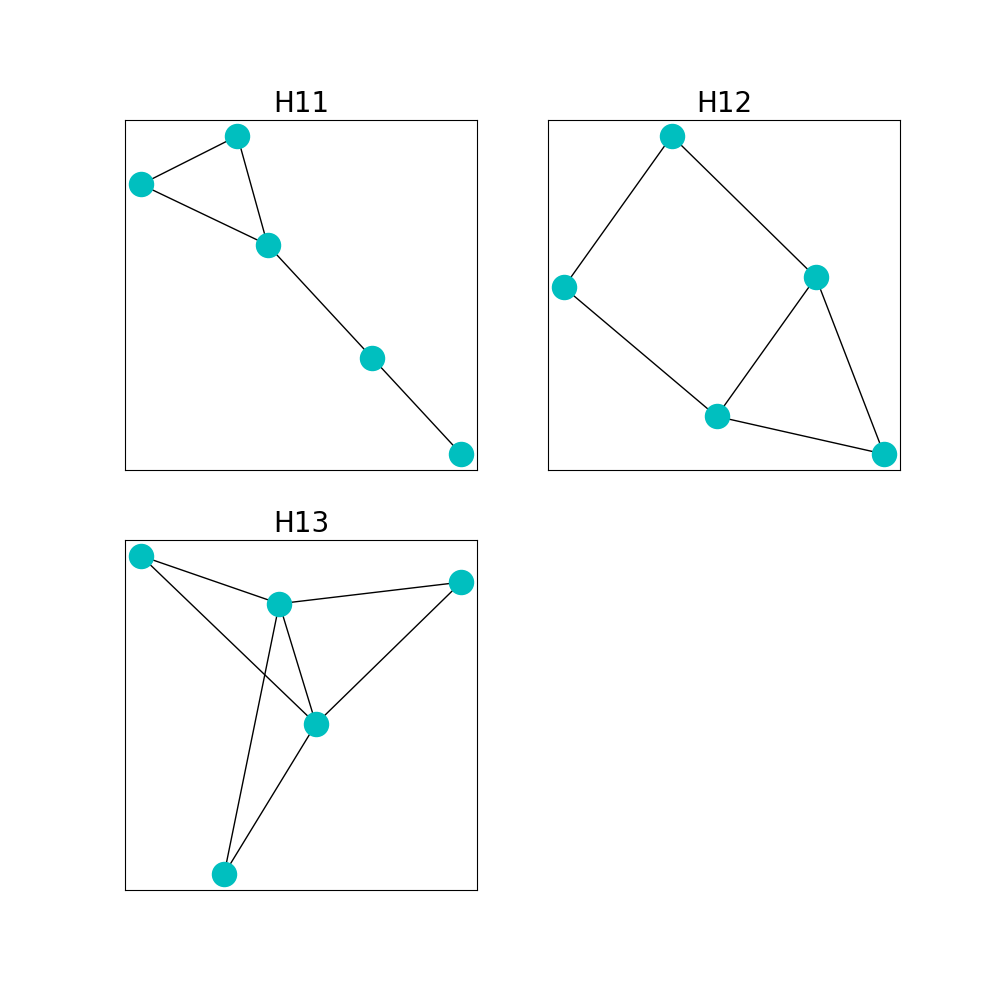
\includegraphics[width=9cm]{Images/motif_set_three.png}
%     \centering
%     \caption{Our last three non-simple motifs}
%     \label{fig:motifs3}
% \end{figure}

\FloatBarrier

\vspace{3mm} 

We will also consider the simple cycles of $C_3$, $C_4$, $C_5$ as motifs. Motif counts can be generated from a network's adjacency matrix in the following ways. Let $A$
be the adjacency matrix of some arbitrary network with greater than four nodes. Let $N_G(M)$ denote 
the total count of motif $M$ in the network described by graph $G$. 

\vspace{3mm}

When counting motifs, we let $E$ denote the set of edges in the network, $e_{i,j}$ denotes a particular edge between the 
$i$th and $j$th nodes. When counting motifs we treat edges as being undirected. $d_i$ denotes the degree of the $i$th node. We define the degree $d_i$ of vertex $v_i$ as the number of 
edges connected to $v_i$. $A$ is the adjacency matrix of the
 graph $G$. Finally, $a^{(k)}_{i,j}$ denotes the $k$th power of the matrix 
element at the $i$th row and $j$th column of matrix $A$. The formulae for motif counts are as follows:

\newpage

\begin{align*}
    &N_G(C_{3}) = \frac{1}{6} \tr({A^3}) \\
    &N_G(C_{4}) = \frac{1}{8} \left(\tr(A^4) -4\sum^{n}_{i=1} {d_i \choose 2} - 2\sum_{i,j \in E} e_{i,j} \right)\\
    &N_G(C_{5}) = \frac{1}{2}\sum_{(i,j)\in E} (d_i - 1)(d_j - 1) - 3 N_{C_{3}} \\
    &N_G(H_{4}) = \sum^{n}_{i=1} {d_i \choose 3} \\
    &N_G(H_{5}) = \frac{1}{2} \sum^{n}_{i=1} a^{(3)}_{i,i} (d_i-2)\\
    &N_G(H_{6})= \sum_{(i,j)\in E}{a^{2}_{i,j} \choose 2 }\\
    &N_G(H_{7}) = \frac{1}{2} \sum^{n}_{i=1} a^{(3)}_{i,i} {{d_i-2} \choose 2}\\
    &N_G(H_{8})= \sum_{(i,j)\in E} a^{(2)}_{i,j} (d_i-2)(d_j-2) - 2 N_G(H_{6})\\
    &N_G(H_{9}) = \sum^{n}_{i-1}(d_i-2) \sum_{j \neq i} {a^{(2)}_{i,j} \choose 2 }\\
    &N_G(H_{10}) = \frac{1}{2}\sum^{n}_{i=1}a^{(3)}_{i,i} \sum_{j \neq i} a^{(2)}_{i,j} - 3 N_G(C_{3})- 2N_G(H_{5}) -4N_G(H_{6})\\
    &N_G(H_{11}) = \sum^{n}_{i=1} {\frac{1}{2}a^{(3)}_{i,i} \choose 2} - 2N_G(H_{6})\\
    &N_G(H_{12}) = \sum_{(i,j)\in E} a^{(2)}_{i,j} a^{(3)}_{i,j} - 9N_G(C_{3}) -2N_G(H_{5})-4N_G(H_{6})\\
    &N_G(H_{13}) = \sum_{(i,j)\in E} {a^{(2)}_{i,j} \choose 3}\\
\end{align*}

We want to understand how each motif count affects another given the addition of new nodes or edges
in any simulation. Some motif graphs contain an appearance of another motif and this will affect how they interact with one another. In Chapter 5, 
an analysis of edge addition on the motif graphs shows simple changes
to a motif's graph may cause a combinatorial effect generating a large number of new motif appearances.

\chapter{Network Theory}

\section{An Introduction}
The social network has taken on new meaning with the advent of the computer, particularly with 
mobile technology. Social media allows for information (and misinformation) to spread rapidly
within and across communities. These communities and their interactions are well-modeled by network theory, an extension of graph theory.
Individuals are represented as nodes in these networks, and their connections as edges. These nodes and their
connections form patterns in a network. These patterns, or motifs, offer
a way to characterize the local structure of the network making the motifs informational features. Motif counts change
over time as users enter and leave the network. The dynamic behavior of these motif counts, and how they correlate with 
one another, offers a way to understand how the network changes locally in time. This analysis can 
extend easily beyond social networks into other domains. In the following section, we first establish 
some of the fundamentals of network theory.


\section{Complex Networks}
The terms ``network" and ``graph" can be used interchangeably as networks are represented
via vertices and edges, but networks are contextual. In its 
most general sense, a network is comprised of objects and connections between them. These
connections may be directed, undirected, weighted - representing any number of different relationships. 
The versatility and effectiveness of this approach has encouraged network modeling in a 
variety of fields: physics, sociology, biology, economy, chemistry \cite{Newman2010}.
Some networks are small and simple. Most networks are large, containing many nodes and connections, many of which are
topologically (or structurally) non-trivial. These we refer to as complex networks, and they are 
commonly found in those fields mentioned previously. 

Complex networks differ from other networks as edges found between vertices 
form in patterns neither completely random nor regular. Such networks often have degree distributions that are fat-tailed,
meaning a few nodes are of relatively high degree, while most nodes are not. These networks
are commonly called scale-free networks. The Barabási–Albert model we examine later falls under
this category. These networks also cluster, which correlates with the scale-free 
property. 

\section{Statistical Properties of Networks}
\label{section: Statistical Properties of Networks}
Network science has many statistical measures to differentiate networks from one another. These
measures offer different levels of insight into a network and its structure.
One such measure is the notion of centrality. There are several different types
of centrality, but each represents a way to denote the most important vertices within a 
given network. One such measure is degree centrality. Given a graph $G$, a vertex $v_i$'s
degree $d_i$ is the number of edges connected to $v_i$.
Aptly named, degree centrality 
assigns a weight to each vertex determined by its degree $d_i$. In Chapter 3 and Chapter 4, degree
centrality is useful as the dynamics of the Barabási–Albert model directly depend on it. The centrality 
measures are informative regarding the connectivity of the network, but leave much to be desired in the way 
of understanding structure.

We make use of the clustering coefficient in Chapters 3 and 4 to characterize graph dynamics. Thij \cite{thij}
notes that clustering coefficients are a way to understand how a network's density changes over time. He 
further notes that future study of the proposed Twitter model in Chapter 4 should include an analysis of its temporal clustering coefficients.
To define the clustering coefficient, we first define the neighborhood $N_i$ of a vertex $v_i$,

$$
N_i = \{v_j: e_{ij}\in E \lor e_{ji} \in E\}
$$

\noindent Where $E$ is the set of edges in the graph. A node $v_i$'s neighborhood is  
the set of nodes, which have an edge between them and $v_i$. The local clustering coefficient of a node $v_i$ in the undirected graph $G$ is defined as 

$$
C_i = \frac{2|p_i|}{k_i(k_i-1)}
$$

\noindent where we define $p_i$

$$
p_i = \{ e_{jk}: v_j, v_k \in N_i, e_{jk}\in E\}
$$

\noindent This can also be calculated by way of the adjacency matrix described in Definition ~\ref{def:adjmat}.

$$
C_i =\frac{1}{k_i(k_i-1)} \sum_{j,k} a_{ij}a_{jk}a_{ik}
$$

\noindent The average clustering coefficient is calculated by arithmetic mean.

$$
{\bar C} = \frac{1}{|V|}\sum_{i} C_i
$$

\noindent The global clustering coefficient is simply

$$
C_{G} = \frac{\text{Total Number of Triangles}}{\text{Total Possible Triangles}}
$$

\noindent Clustering allows us to understand how dense a network is relative to a complete graph. 

\section{The Social Network Twitter}
\label{section:Twitter}
Twitter is now, as of 2021, an eminent example of complex networks in social media.
As of 2019, there are 330 million monthly active users on Twitter, thirteen years after the platform was
established in 2006. However, according to Pew Research, the top ten percent of Twitter users tweet 138 
tweets per month, while the bottom ninety percent of Twitter users only tweet twice per month. The top ten percent of users
have a median of 387 followers, while the bottom ninety percent have only a median of 19 followers. The top ten percent
also follow more users, a median of 456 accounts, compared to a median of 74 accounts for the bottom ninety percent \cite{wojcik2019sizing}.
This itself is suggestive of Twitter being a scale-free network, but analysis confirms this \cite{Aparicio}. Twitter, as
a network, exhibits a fat-tailed degree distribution. Moreover, its estimated
average clustering coefficient is 256,000 times larger than expected for a random graph.

Twitter's status as a complex network aside, the platform is also notable for its position among social networks not only for its size,
but also its influence on culture and politics. During the 2016 election, a survey of
thirty million tweets from two million users, linked articles that were found to be spreading
false information. Moreover, this information spread based on community structure within an inclusive left-right
influencer network. Twitter is cliquey and the communities form around 
shared interests. In online communities where exposure to the same memetic theme occurs frequently, both
facts and rumors may spread easily and quickly \cite{bessi}.

Twitter also has a substantial economic impact. Twitter sentiment is known to precede fluctuations
in the stock market \cite{Bollen2011} and Bitcoin prices \cite{bitcoin}. However, only a handful of Twitter users actually have influence  
(although groups of people could theoretically be enough to influence market prices \cite{stonks}).
Elon Musk is one such person who, as of March 2021, has influenced multiple markets driving Tesla's share
price up and down \cite{elontweet}, as well as causing jumps in cryptocurrency prices  \cite{elontweet2} \cite{dogecoin}. Musk, 
is as of 2021, the forty-third largest Twitter account, giving him much more influence than the vast majority of users.

Twitter's suitability as a subject of network science is clear. The users and followers (and retweets) are naturally 
described by vertices and edges. One can generate networks from Twitter in two ways.
 First, there are the user accounts which are linked to one another through 
followers and follows, in-degrees and out-degrees. An example of this is given in Figure~\ref{fig:elon_graph}. One can also construct networks
of tweets and retweets as discussed in Chapter 4. A user posts a message, which is  
retweeted by a portion of their followers, which is then again retweeted by a portion of their followers.
 It is this latter case we will consider in the Thij model.

 \begin{figure}
    \centering
        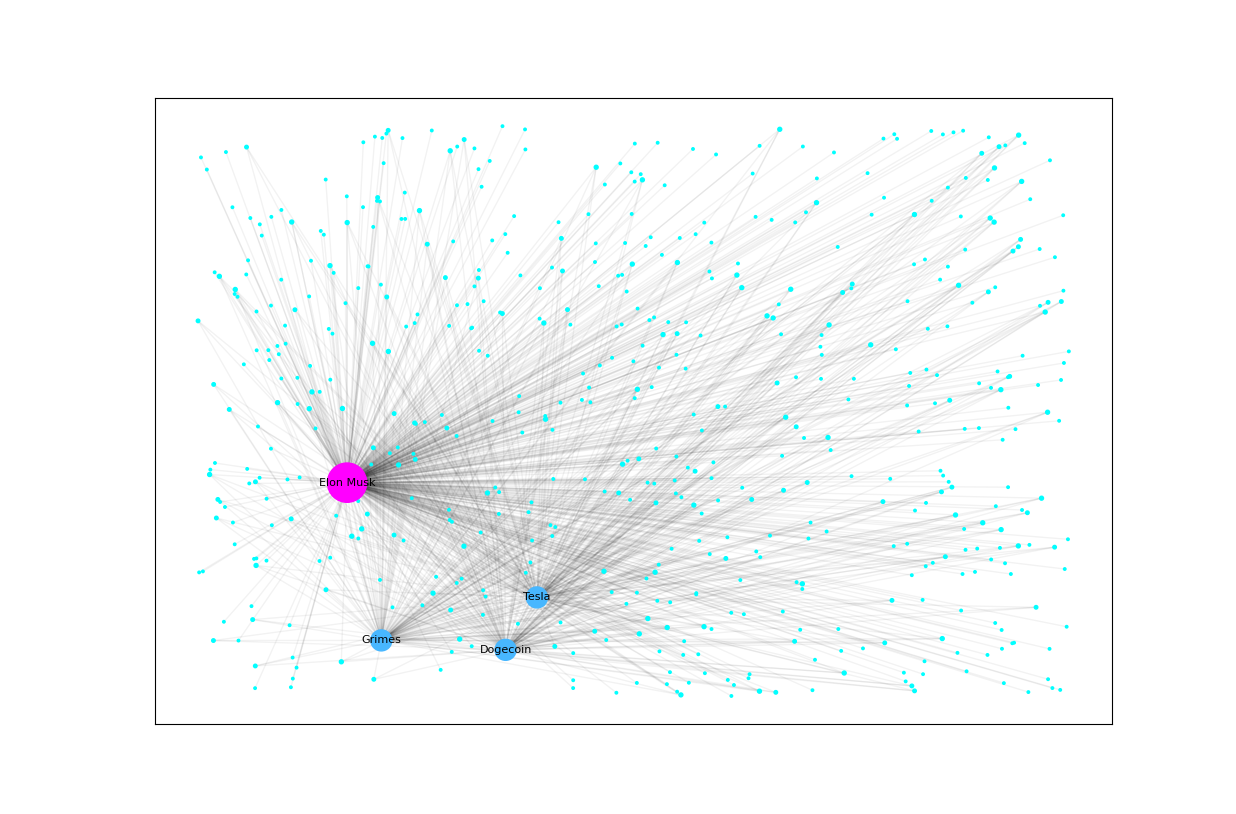
\includegraphics[width=15cm]{Images/elon_graph.png}
        \caption{All the circles represent nodes or users in this Twitter network. The edges between the nodes denote follows.
         The red node is a single user in the Twitter network following Tesla, Dogecoin, and Grimes (denoted by the red edges), but no others. The 
        red user receives all tweets and retweets from Tesla, Dogecoin, and Grimes. This user may retweet these messages
        outside the network, potentially bringing in more users to the network. Note, the red node and its adjacents are isomorphic to $S_3$ (or the $H_{4}$ motif). \label{fig:elon_graph}}
\end{figure}

\chapter{Barabási–Albert Model}
\label{section:BA model}
The early models of networks failed to capture the characteristics that appear in empirical data. An
 early model proposed by Paul Erdős and Alfréd Rényi, appropriately called the Erdős–Rényi model, generates
graphs of fixed node count where each pair of nodes has the same probability to have an edge between them \cite{Erdoes}. 
Réka Albert and Albert Barabási proposed the Erdős–Rényi model 
lacked key pheonmena of most real-world networks \cite{barabasi2016network}.
 First, real networks often have degree distributions 
that are not explainable by the degree distribution of the Erdoes-Renyi model.
Second, real networks have a sizable largest connected component - a large cluster 
of nodes inside the network, forming a hub of activity.
 Finally, the local clustering coefficient of most networks
decreases as the node degree decreases, but is independent of overall graph size.
Réka Albert and Albert Barabási developed a model of complex networks 
encompassing those we find common in practice.
Edges are made to follow a preferential attachment
mechanism, which ascribes probabilities of attachment by the relative degree of the nodes in a network. 
It is a point of contentious debate if networks are scale-free and their degree distributions follow a power-law.
A network is said to follow a power-law if the fraction of nodes $P$ having $k$ edges is 

$$
P(k) \approx k^{-\gamma} 
$$

\noindent The preferential attachment mechanism of the Barabási–Albert model generates this power-law. 
The Barabási–Albert model typically exhibits $2<\gamma<3$.
%%%%%% Left off editing here

To model such a network, we begin at $t=0$ by initializing $m$ nodes and randomly distribute a number of edges between them
according to a uniform distribution. Then at each time-step $t > 0$, we introduce a new node 
and $k$ edges between that node and the existing nodes. We assign probabilities of attachment to the $n$th node via the
 probability distribution:

$$
\Pi(n) = \frac{d_n}{\sum^{N}_{i=1} d_i}
$$

\noindent where $d_n$ is the degree of the $n$th node and $N$ is the total number of nodes at $t-1$.
 Nodes which have a high degree are probabilistically more likely to be attached to new nodes. 

In Figure~\ref{fig:BA1}, we see that only certain motifs can be generated in the $k=1$ BA model.
Motif counts in the Barabási–Albert model are dependent upon the initialization of the $m$ nodes 
and the choice of $k$. For example, if $k=1$ the model cannot complete any new cycles. If the
intial graph at $t=0$ does not contain any $C_3$ or $C_4$ appearances, then any motif 
which has an induced subgraph isomorphic to $C_3$ or $C_4$ cannot appear. The BA model 
for $k=1$ can only attach nodes to the existing  $C_3$ or $C_4$ appearances and in that 
way generate new $H_{7}$, $H_{8}$, or $H_{9}$ appearances. The BA model with $k=2$ is capable of generating those
 new $C_3$, $C_4$, and $C_5$ appearances in the network quite easily as seen in Figure~\ref{fig:BA2}.

\begin{figure*}[h!]
    \includegraphics[width=\linewidth]{Images/pref_attach_1_counts.png}
    \centering
    \caption{This Barabási–Albert model is initialized with $m=8$ nodes.
    At each time-step a new node enters and is attached to $k=1$ nodes by the preferential attachment mechanism.
      All simulations are terminated after the network reaches a size of $300$ nodes.}
    \label{fig:BA1}
\end{figure*}


\begin{figure*}[h!]
    \includegraphics[width=14cm]{Images/graph_stats_pref_attach_8_1_300.png}
    \centering
    \caption{Statistics characterizing the development of the Barabási–Albert model for $k=1$.
    Edges and nodes grow linearly. We also see as Barabási noted, the edge density and clustering coefficients decrease asymptotically.}
\end{figure*}


\begin{figure*}
    \includegraphics[width=14cm]{Images/final_pref1_centrality.png}
    \centering
    \caption{The Barabási–Albert model for $k=1$ at the final time-step. The color and size of the nodes reflect
            the degree centrality of each node.}
\end{figure*}

\begin{figure*}[h!]
    \includegraphics[width=\linewidth]{Images/pref_attach_2_counts.png}
    \centering
    \caption{This Barabási–Albert model is initialized with $m=5$ nodes.
    At each time-step a new node enters and is attached to $k=2$ nodes. We see that different motif appearances
    correlate for the $k=2$ simulation and other motif appearances, like those of $C_3$ and $C_5$, can be generated.}
    \label{fig:BA2}
\end{figure*}

\begin{figure*}[h!]
    \includegraphics[width=14cm]{Images/graph_stats_pref_attach_10_2_300.png}
    \centering
    \caption{Statistics characterizing the development of the Barabási–Albert model for $k=2$.
    Edges and nodes grow linearly, with 2 edges added at each time-step. The clustering coefficients asymptotically
    approach zero. The histogram at
    the final time shows the vast majority of nodes, approximately 220, have two or three attachments
    while three vertices have a degree greater than $35$.}
\end{figure*}

\begin{figure*}
    \includegraphics[width=14cm]{Images/final_pref2_centrality.png}
    \centering
    \caption{The Barabási–Albert model for $k=2$ at the final time-step. Once again the color and size
            reflect the degree-centrality of each node.}
\end{figure*}

% The Barabási–Albert model exhibits a few characteristics that differentiate it from the 
% Erdős–Rényi model. If we consider its diameter, the maximum distance in the network,
% for $k>1$ and sufficiently large time, we can write the diameter analytically. Let $N$ be the 
% total number of nodes in the network.

% $$\text{diam}(G) = \frac{\ln(N)}{\ln(\ln (N))}$$

% The diameter grows slower than $\ln(N)$ or the rate of growth for the
% Erdős–Rényi model's diameter. We can also examine the clustering coefficient of the model. 
% The clustering coefficients for the preferential attachment model grows according to \cite{klemm_2002},

% $$
% C(G) = \frac{(\ln (N))^2}{N}
% $$

% This differs from the Erdős–Rényi model by the term $(\ln (N))^2$,
% which increases the clustering coefficient for large $N$. Still, as $N$ grows large,
% both clustering coefficients
% decrease, asymptotically approaching zero. The Barabási-Albert network is locally
%  more clustered than a random network for all $N$ \cite{barabasi2016network}.

The Barabási–Albert model is a good candidate to as a base-line to our more complex model.
 The Barabási–Albert model 
represents a simpler, non-trivial model, which is widely acknowledged as a useful tool
for understanding networks across a variety of disciplines. The preferential attachment mechansim 
only allows for the addition of nodes and a set number of edges at teach timestep.There are 
limitations to the Barabási–Albert model. The nodes and edges are restricted to linear growth, which
may fail to capture certain phenomena that appear empirically. The model is also incapable
 of removing nodes, a point on which Barabási himself has elaborated. Our next model
 does account for the first of these limitations at the cost of increased complexity.

\chapter{The Thij Model}
\label{section:Thij model}
The Thij model is a particular random graph that seeks to model the development of a Twitter network 
 \cite{thij}. Twitter offers a platform where a user may post a message
to all of their followers' feeds. Those followers may then ignore, like, reply (comment), or retweet (quote tweet) that message. In the
instance they choose to retweet the message, that message is then posted to their respective feed and their own
followers now have the opportunity to retweet that same message. If a
message has received a significant number of retweets the message is more likely to be seen and thus
retweeted again. A preferential attachment mechanism drives the popularity of the most popular tweets \cite{Aparicio}. The 
Thij model incorporates a superstar mechanism that was first proposed in \cite{Bhamidi_2015}. The superstar mechanism is 
ascribed to original tweets which have much higher chance of being retweeted within a network.

A user can retweet different original messages at different times, meaning edges can be generated between
existing nodes in the network. Accounting for this, one can produce
a model better suited to Twitter simulations than the Barabási–Albert model described in Chapter 3.

We wish to simulate a network of retweets. There are original message nodes from users $u_i$ and retweets from users $v_i$. All users
are capable of retweeting or posting original messages. 
 The simulation starts with an initial message node from user $u_{0}$ at time $t=0$. For all time-steps, there is now the possibility of three events: $T1$,
$T2$, and $T3$. 

\vspace{3mm}

\noindent $\pmb{T1}$: A new message node from user $u_k$ appears.

\vspace{3mm}

\noindent $\pmb{T2}$: A user $v_k$ enters the retweet network and retweets an existing user's message. The retweeted message is either an original message node $u_i$
or another user $v_i$'s retweet. This user $v_k$ retweets an original message node $u_i$ with 
probability $q$ and any other node with probability $\frac{1-q}{N}$. $N$ is the total number of nodes in the network.

\vspace{3mm}

\noindent $\pmb{T3}$: An existing user $v_i$ retweets another existing user $u_i$ or $v_j$. The retweeter retweets a message node with probability 
$q$ and all other message or retweet nodes with probability $\frac{1-q}{N}$.

\vspace{3mm}

For clarity, we make a distinction between the posts of original messages and retweets.
$v_i$ may be a simple retweet, or a quote tweet, meaning $v_i$ may reasonably retweet $v_k$ who may have added commentary to the original message.
We must also note that there will be multiple message nodes in the retweet graph, and thus
 we have to decide for any given event
which particular message node should be assigned the $q$ probability.
 Here we introduce a preferential attachment mechanism. At any time $t$,
given a $T2$ or $T3$ event occurring, the probability of a particular message node being chosen is almost the
same mechanism described in the Barabási–Albert model. Instead, a message node is chosen
by its total descendants and not by the degree of the message node itself. In essence, a message node
is selected based upon the number of those who have retweeted the message and all those who have retweeted
retweets of that message.


We now must assign probabilities of $T1$, $T2$, and $T3$ events. Let $P(T_i)$ denote probability of event $T_i$.
Let $\lambda$, and $p$ be parameters such that $\lambda \geq 0$, and $1 \geq p \geq 0$. 

\begin{align*}
    &P(T1) = \frac{\lambda}{1 + \lambda} \\
    &P(T2) = \frac{p}{1 + \lambda} \\
    &P(T3) = \frac{1-p}{1 + \lambda} \\
\end{align*}

\begin{figure*}
    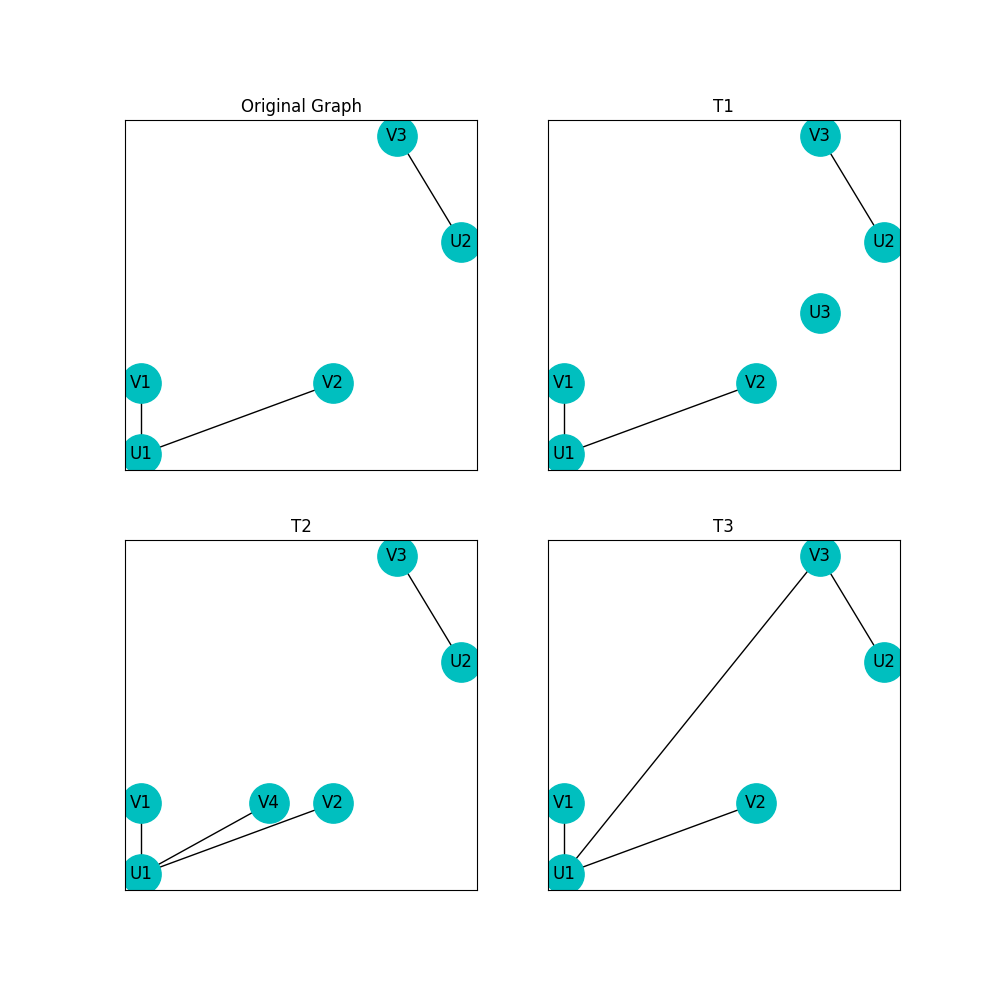
\includegraphics[width=12cm]{Images/events.png}\
    \centering
    \caption{We see the $T1$, $T2$, and $T3$ events on a simple graph. In the $T1$ case 
    we see a new message node $U3$ appears. It has yet to be connected to anything at all. In $T2$
    we see a new node $V4$. This is a retweet of the message $U1$. Finally in the last plot we see
    a $T3$ event. Here the user $V3$, who has already retweeted $U2$, now retweets message $U1$.}
\end{figure*}

Our choices of $\lambda$ and $p$ will drastically affect the dynamics of the graph, as well as the motif counts that make
up its structure. We want to consider a series of cases for different probabilities allowing us to make informed predictions about the graph's development over time.
The motif counts for various parameters help demonstrate the differences in scale 
and structure which arise from different probability distributions. Consider the case when $0.5 > \lambda > 0$ and $0.5 \gg p > 0$. In this case, it is the $T3$ event
expected to be the most prevalent. For these parameter values, we see in Figure ~\ref{fig:thij0202} the first four greatest motif counts almost 
everywhere in order are $H_{7}$, $H_{8}$, $H_{9}$, and $H_{10}$. The $T3$ mechanism allows for more $C_3$'s and $C_4$'s to form within the network.

Next, consider $1>\lambda>0.5$ and $0.5 \gg p > 0$. Here the $T1$ event should dominate the dynamics
with many new message nodes introduced to the overall retweet network. In this scenario, we have
a greater likelihood of $T3$ events over $T2$ events. This means those nodes without connections are likely to become connected to other nodes. In Figures
~\ref{fig:thij0802} and ~\ref{fig:network0802}, we can visualize the motif development and the overall network. Looking at the final time degree
distribution in Figure~\ref{fig:stats0802}, we see the majority of nodes are still unconnected.

What about the case $0.5 \gg \lambda > 0$ and $1 > p \gg 0.5$? The probability distribution is such that adding a new node
with an edge is the most likely outcome. These parameter choices combined with the superstar parameter $q=0.9$ implies that $T2$ and $T3$
attachments are very likely to target the root message node. In Figure~\ref{fig:thij0208}, we see the resulting star pattern in the motif counts 
and the end-result in Figure ~\ref{fig:network0208}.The preferential attachment mechanism encourages
an induced subgraph $S_{k}$ to form with $k\gg 1$. For any $k \gg 3$, $S_{k}$
contains many appearances of $H_{4}$. For every increase in $k$, another increase becomes more likely.

Last, $1>\lambda>0.5$ and $1>p\gg0.5$, we see an increased chance of adding
many new root messages, but still a good possibility of introducing a new node with a new edge, but a decreased possibility of 
adding in only new edges. For an example of the resulting motif counts we can look to Figure~\ref{fig:thij0808}. 

% \clearpage

\begin{figure*}[h!]
    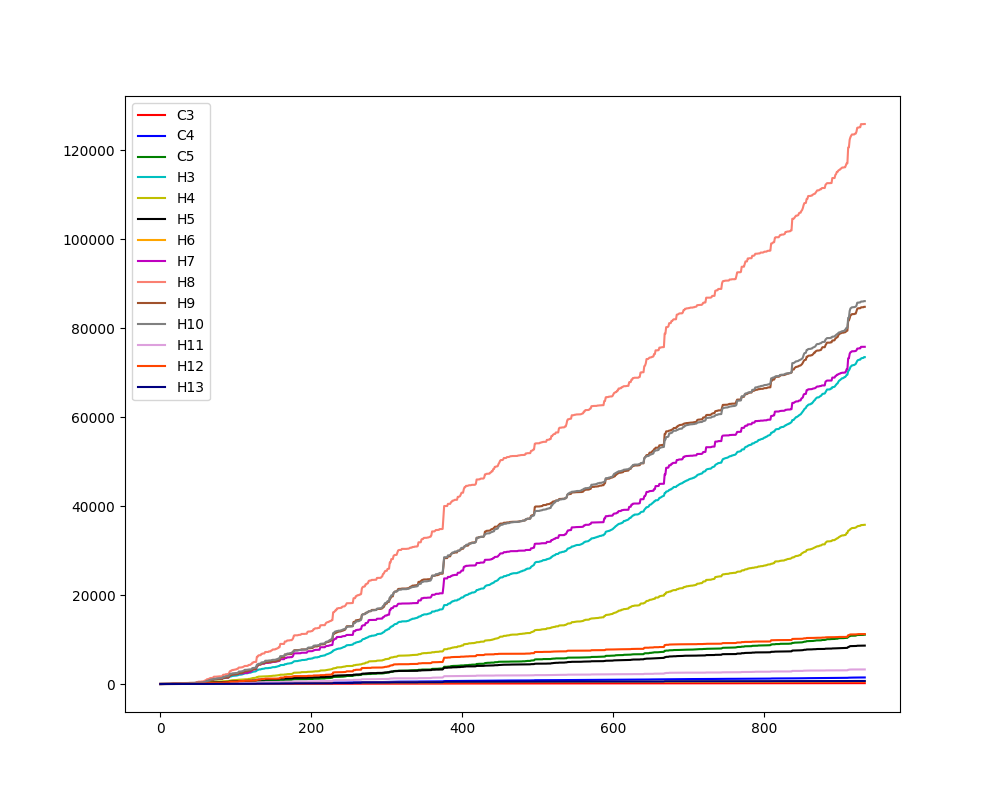
\includegraphics[width=15cm]{Images/twitter_sim_for_stats_3_0.2_0.2.png}
    \centering
    \caption{Here, for $\lambda=0.2, p=0.2$, we see that $H_{8}$'s lead with $H_{9}$'s and $H_{10}$'s. These motifs are
     closely correlated with one another throughout the time series. $H_{7}$'s
    and $H_{3}$'s have the next highest counts where $H_{7}$ movement prima facie
    appears to correlate with $H_{8}$ counts, while $H_{3}$ counts steadily increases throughout time.}
    \label{fig:thij0202}
\end{figure*}

\begin{figure*}[h!]
    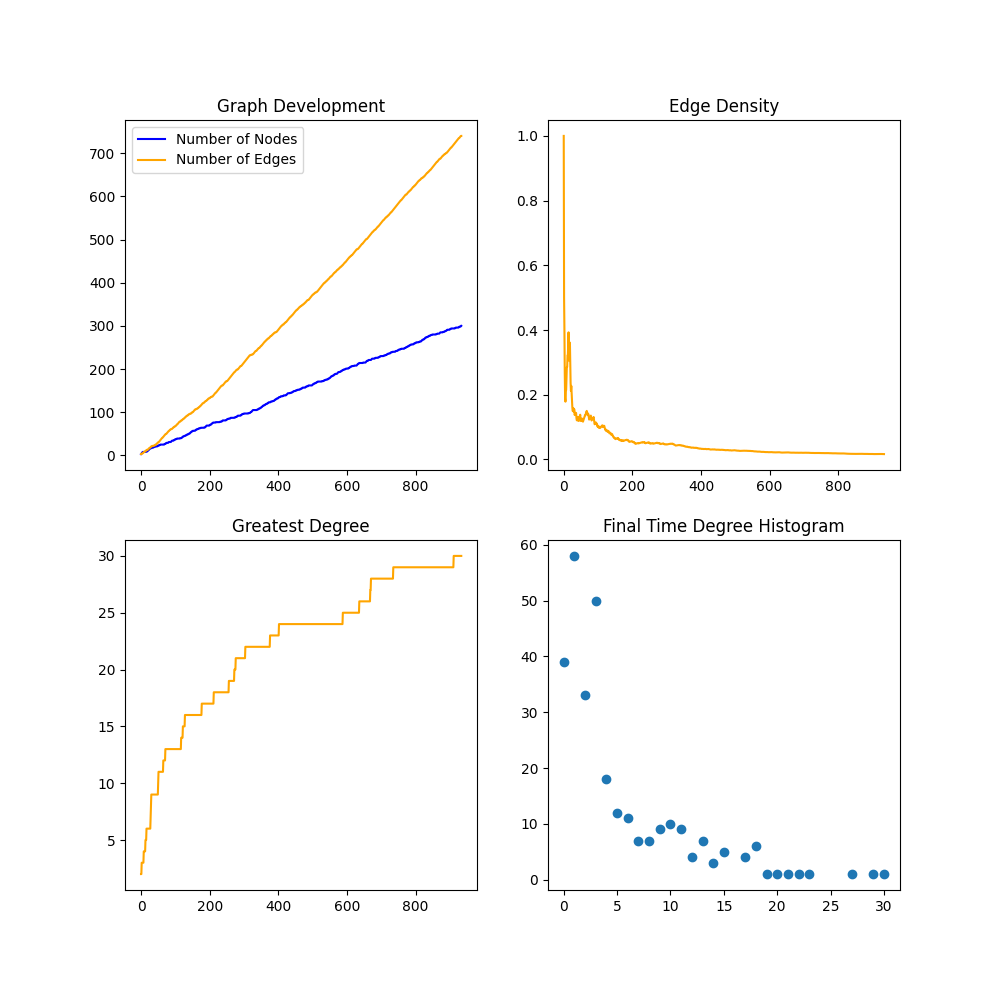
\includegraphics[width=14cm]{Images/twitter_sim_stats_3_0.2_0.2.png}
    \centering
    \caption{Compared to the Barabási–Albert model, for the Thij simulation neither edge count nor node
     count must grow strictly linear at each time-step. The edge density tends toward
     zero, although a $T3$ event amounts to a small increase in edge density. The clustering 
     coefficients tend towarx zero asymptotically, but are surprisingly large early in the simulation. Finally, we 
    see a final time degree histogram that is similar.}
\end{figure*}

\begin{figure*}[h!]
    \includegraphics[width=14cm]{Images/final_Thij_centrality_0202.png}
    \centering
    \caption{The network for $\lambda=0.2$, $p=0.2$ at the final time-step.}
\end{figure*}

\clearpage

\begin{figure*}[h!]
    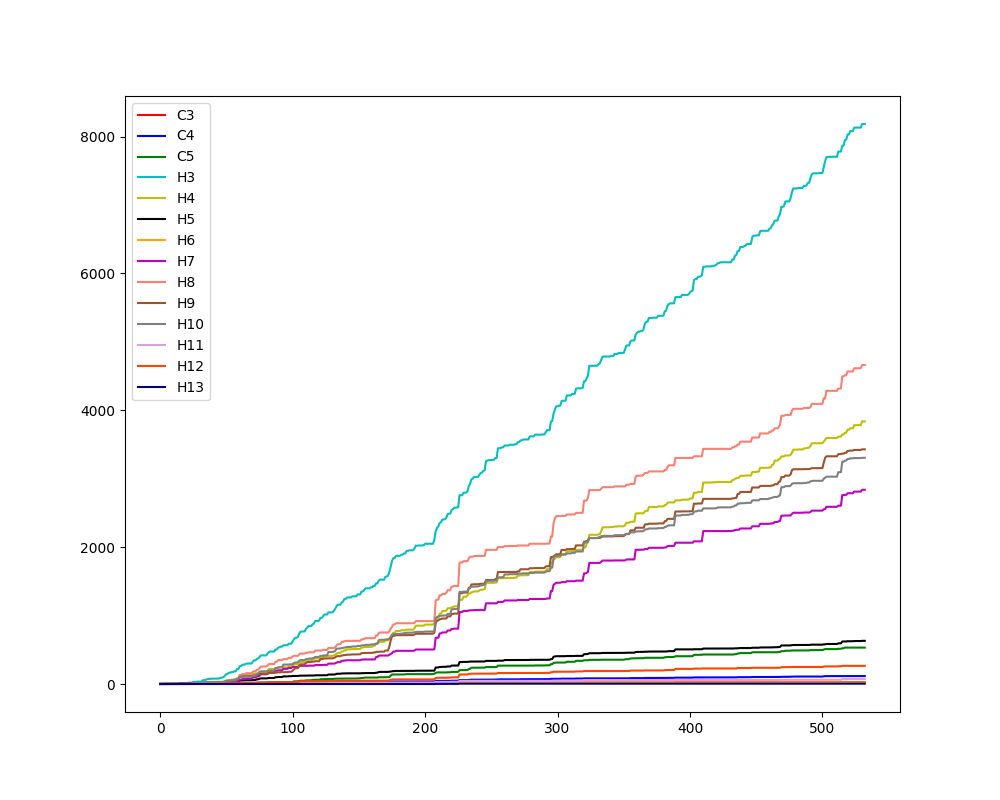
\includegraphics[width=15cm]{Images/twitter_sim_for_stats_3_0.8_0.2.png}
    \centering
    \caption{For $\lambda=0.8, p=0.2$ many new message nodes appear ($T1$ events), but
    with low $p$ we should see many $T3$ events connecting these nodes. $H_{3}$ motifs are the most prevalent
    followed by $H_{8}$'s and $H_{4}$'s.}
    \label{fig:thij0802}
\end{figure*}

\begin{figure*}[h!]
    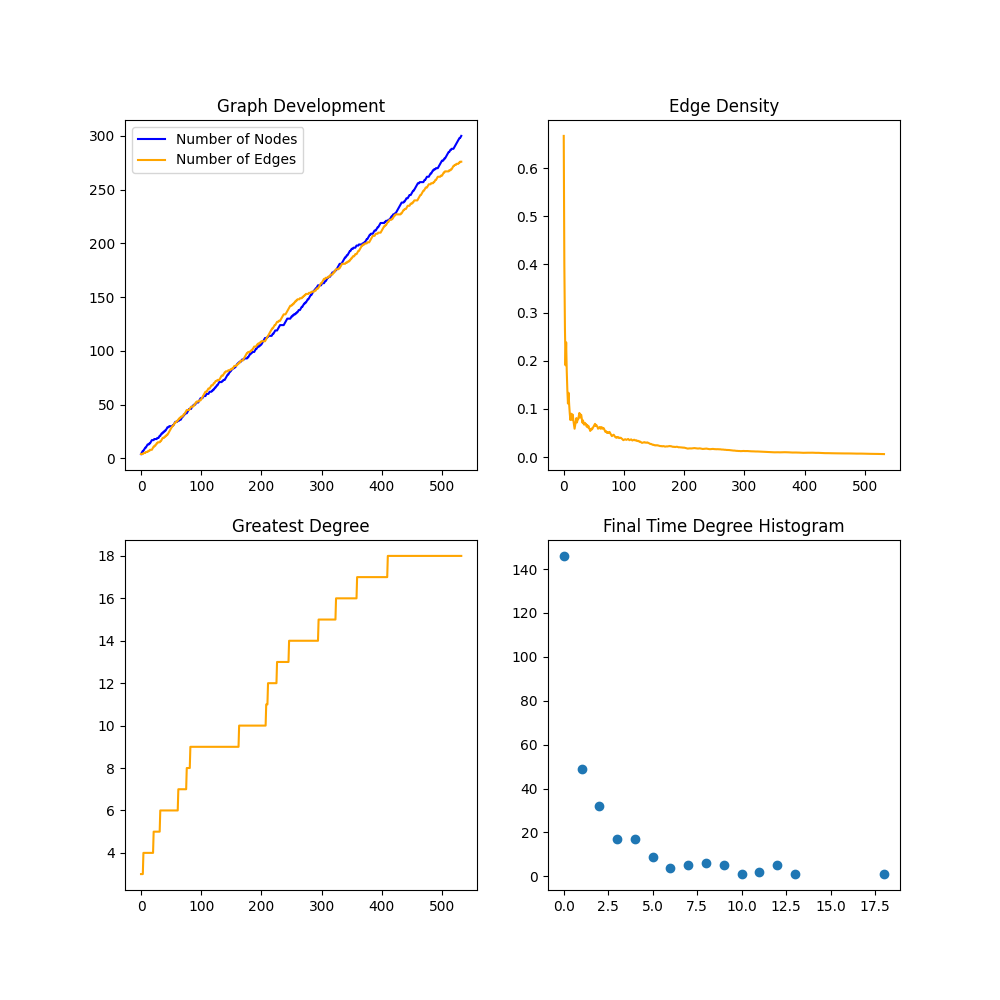
\includegraphics[width=14cm]{Images/twitter_sim_stats_3_0.8_0.2.png}
    \centering
    \caption{For $\lambda=0.8, p=0.2$, edges and nodes travel tightly together with roughly a ratio of 
     one-to-one. Here we see many nodes unattached with degree zero.
    For those that are attached, we do see a power law describing degree distribution, but one that is not quite
    as strong as those found in other simulations.}
    \label{fig:stats0802}
\end{figure*}


\begin{figure*}[h!]
    \includegraphics[width=14cm]{Images/final_Thij_centrality_0802.png}
    \centering
    \caption{The network for $\lambda=0.8$, $p=0.2$ at the final time-step.}
    \label{fig:network0802}
\end{figure*}

\clearpage

\begin{figure*}[h!]
    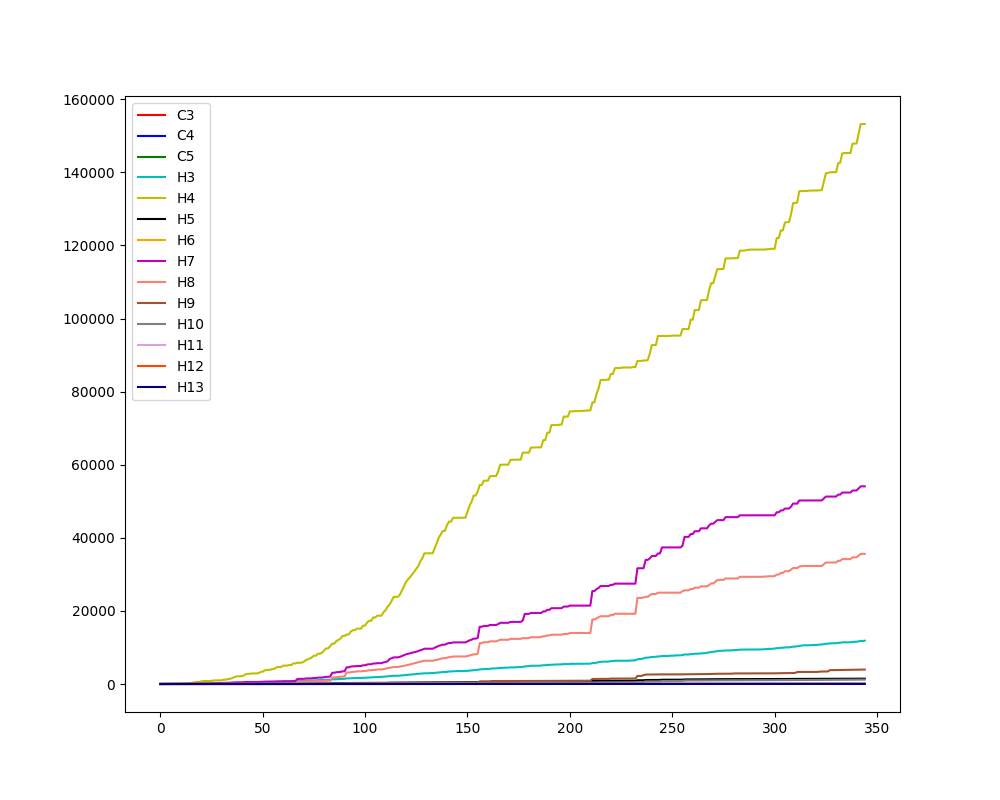
\includegraphics[width=\linewidth]{Images/twitter_sim_for_stats_3_0.2_0.8.png}
    \centering
    \caption{For the parameter values $\lambda=0.2, p=0.8$, there is a decreased likelihood of new message nodes appearing, but 
    high $p$ means a greater likelihood of $T2$ events which we speculate lead to a large
    count of $H_{4}$'s. $C_3$'s exist around the center where all these $H_{4}$'s
    overlap. Although $C_{3}$'s are not prevalent here, a combinatorial explosion generates 
    many $H_{7}$'s and $H_{4}$'s. This is discussed further in Chapter 5.}
    \label{fig:thij0208}
\end{figure*}


\begin{figure*}[h!]
    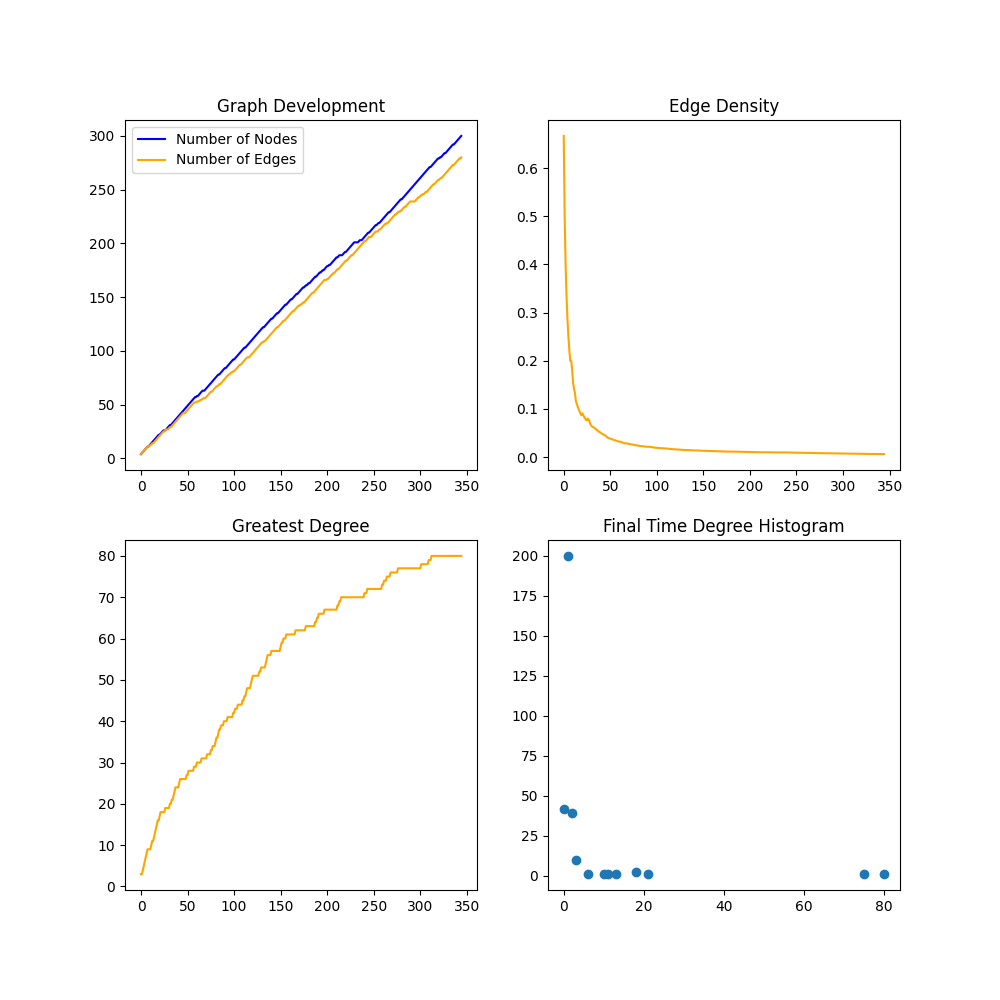
\includegraphics[width=14cm]{Images/twitter_sim_stats_3_0.2_0.8.png}
    \centering
    \caption{For $\lambda=0.2, p=0.8$, we see two nodes with degrees greater than seventy
    but an abundance of nodes with only one or two connections. We can see this 
    reflected in the graph of the network in figure~\ref{fig:network0208}. }
    \label{fig:twittersim28}
\end{figure*}


\begin{figure*}[h!]
    \includegraphics[width=14cm]{Images/final_Thij_centrality_0208.png}
    \centering
    \caption{The network for $\lambda=0.2$, $p=0.8$ at the final time-step.}
    \label{fig:network0208}
\end{figure*}

\clearpage

\begin{figure*}[h!]
    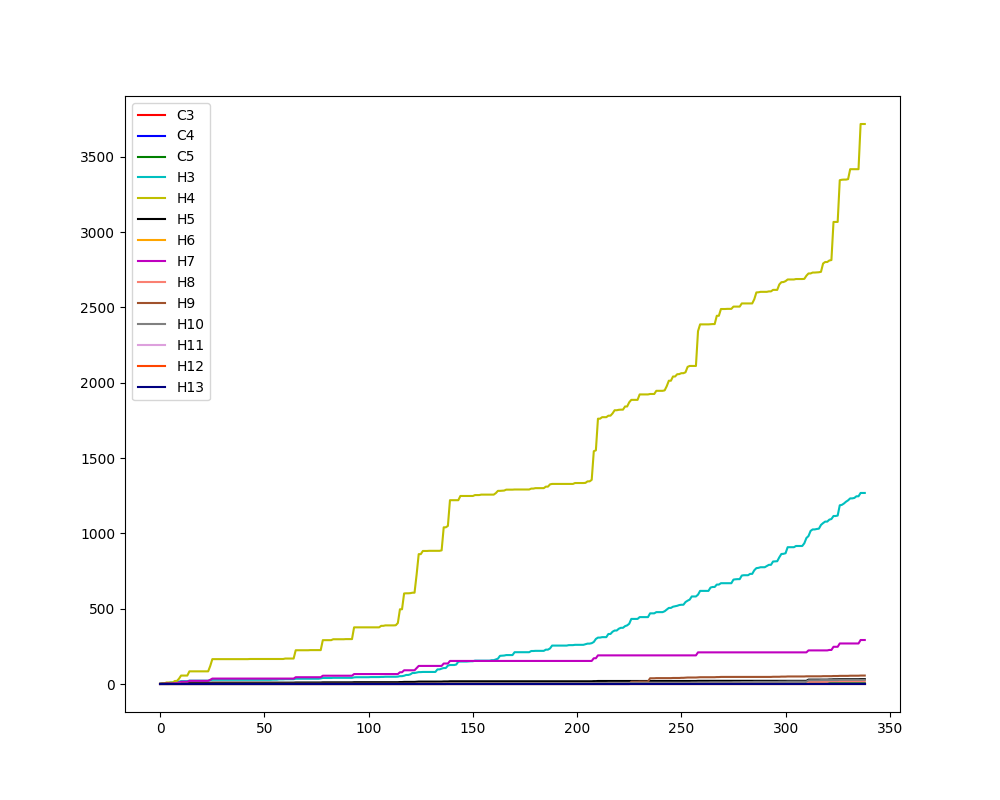
\includegraphics[width=\linewidth]{Images/twitter_sim_for_stats_3_0.8_0.8.png}
    \centering
    \caption{For $\lambda=0.8, p=0.8$, like the simulation in figure ~\ref{fig:twittersim28}, we see a prominence of $H_{4}$'s.
     The scales of the motif counts between simulations are separated by several orders of magnitude. In this simulation,
    there is a relatively high count of $H_{3}$'s. We can explain the difference in magnitude
     due to many $T1$ events introducing many unconnected nodes, but the occurrence of $T2$ events 
     is sufficient to make $H_{4}$ the motif of highest count.}
     \label{fig:thij0808}
\end{figure*}

\begin{figure*}[h!]
    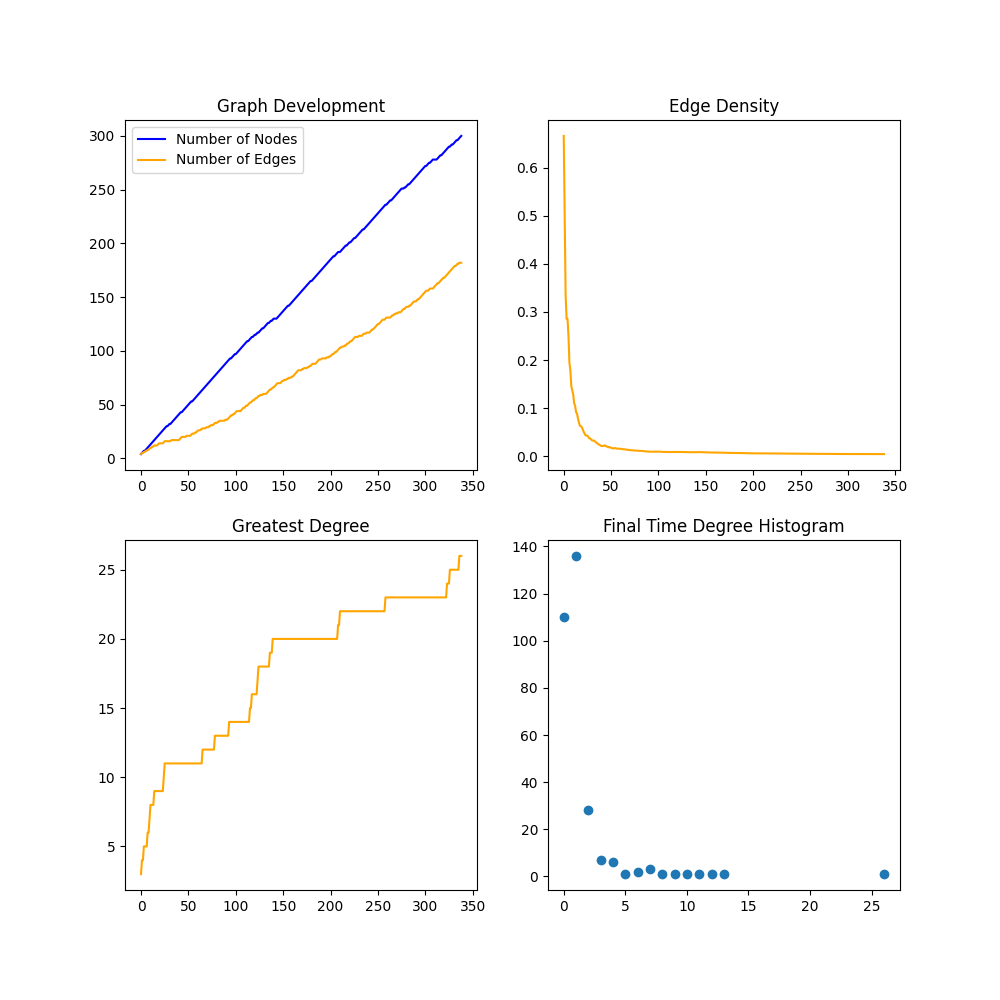
\includegraphics[width=14cm]{Images/twitter_sim_stats_3_0.8_0.8.png}
    \centering
    \caption{The $\lambda=0.8, p=0.8$ Twitter simulation produces many more nodes than 
    edges, because of the frequency of $T1$ events. The vast majority of nodes only 
    have degrees of one or two, while we see a single node with 25 connections.
    This might suggest many small clusters of nodes with a single larger
    cluster around a single message node. The clustering coefficient suggest a low number 
    of triangles within the graph.}
\end{figure*}


\begin{figure*}[h!]
    \includegraphics[width=14cm]{Images/final_Thij_centrality_0808.png}
    \centering
    \caption{The network for $\lambda=0.8$, $p=0.8$ at the final time-step.}
\end{figure*}

\clearpage

The dynamics and end state of the network vary across parameter choices.
Given greater $p$ values and smaller $\lambda$ values a few nodes exhibit relatively large degree distributions. The ratio of edges to vertices for the Twitter model varies much more than the Barabási-Albert model.
This is expected given the probabilistic nature of how many edges may be added in a given turn (0 or 1) compared
to the given $k$ edges of the Barabási–Albert model. This ratio affects not only the network structure but the time-scale 
over which the network node count grows.

Each graph spans over \textit{very} different
time frames. Each graph was allowed to grow to a maximum of three hundred nodes before ending the simulation. Ending the simulation with a size
threshold makes a comparison of the network topology more feasible. For $\lambda=0.2$ and $p=0.8$, the model was able to reach 
three-hundred nodes very quickly, in approximately three-hundred time-steps, whereas for $\lambda=0.2$, $p=0.2$ it took nearly a thousand time-steps. 
This is a consequence of $\lambda$ controlling the frequency of a new node entering without a new edge and
$p$ controlling the frequency of new nodes added with edges or if only new edges are introduced. 

\chapter{Barabási–Albert Model Motif and Thij \texorpdfstring{$\bf T2$}{T2} Event Motif Dynamics}

To gain insight into graph dynamics, we analyze how the composition of a motif's graph changes 
upon the addition of a node to a given motif, and attaching that node to an existing node. 
The tables below count the appearances of a motif in the respective graphs.
For example in Figure ~\ref{fig:H4T2}, after adding a node to the root of $S_3$ or $H_{4}$, we count four appearances 
of $H_{4}$ as the motif $H_{4}$ is isomorphic to four induced subgraphs in the newly generated motif. 

\section{The \texorpdfstring{$H_{3}$}{H3} Motif}
We begin by considering the $H_{3}$ motif. The $H_{3}$ motif is simply a four-path. A preferential attachment
mechanism on this motif will most likely connect a new node to one of the center nodes with probability
$0.67$, and to an outer node with a probability of $0.33$. In the Thij model,
this change is based upon which node has the superstar quality. 

\begin{figure}[!ht]
    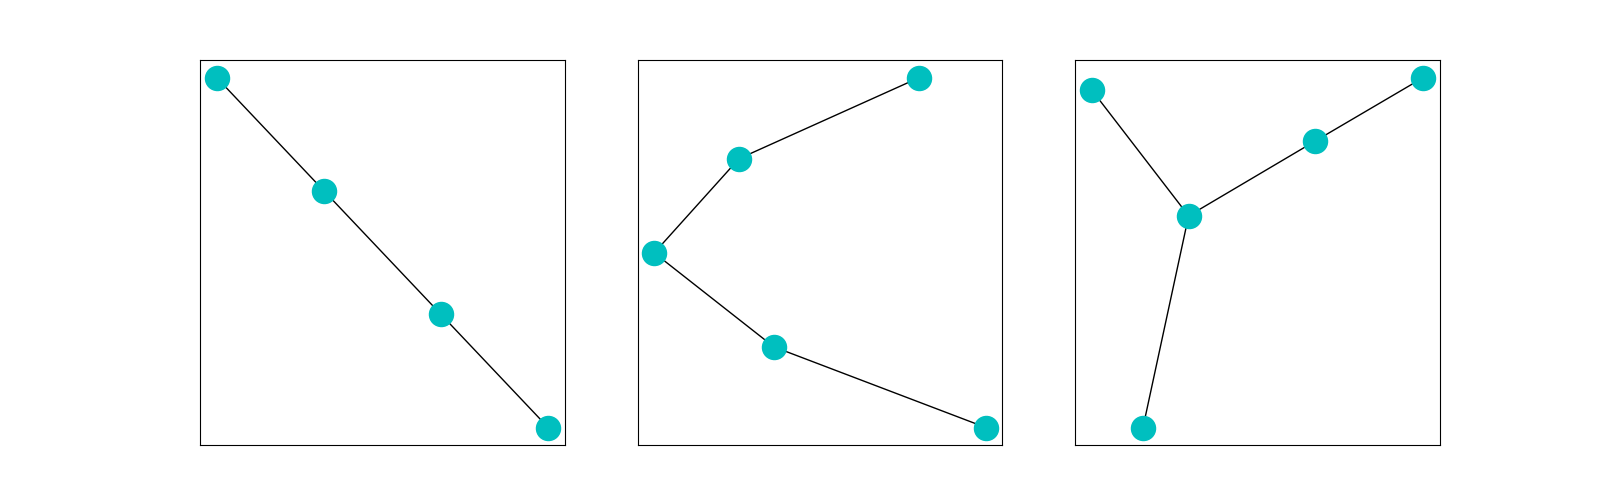
\includegraphics[width=\linewidth]{Images/H3_evolution.png}
    \centering
    \caption{The possible graphs generated by adding a node to the $H_{3}$ graph 
    and connecting it to an existing node.}
\end{figure}
\FloatBarrier

\begin{table}[h!]
    \centering
        \begin{tabular}{||c c c c||} 
            \hline
            Motif Count & Original Motif & Event 1 & Event 2\\ [0.5ex] 
            \hline\hline
            $H_{3}$ & 1 & 2 & 2\\ 
            \hline
            $H_{4}$ & 0 & 0 & 1\\
            \hline
        \end{tabular}
        \caption{The rows denote counts of isomorphisms that can be found in either 
        motif. The $H_{3}$, a four walk, can be found twice in the first event or second event.}
        \label{table:1}
\end{table}

\section{The \texorpdfstring{$H_{4}$}{H4} Motif}
The $H_{4}$ motif is one of the motifs that are of primary interest given that for any star $S_k$
with $k \geq 3$ we will find ${k \choose 3}$ appearances of the motif. Given an induced subgraph isomorphic to the star $S_k$,
attaching a node to the root node of $S_k$ will generate $k$ new appearances of the $H_4$ motif. For large
clusters of $H_{4}$ motifs the $H_{4}$ motif count will grow rapidly in time. The probability
for the first event on the original motif is $0.5$, and for the second event $0.5$. A significant
difference in the occurrence of the first event over the second event will encourage more of the first event in the future. 

\begin{figure}[!ht]
    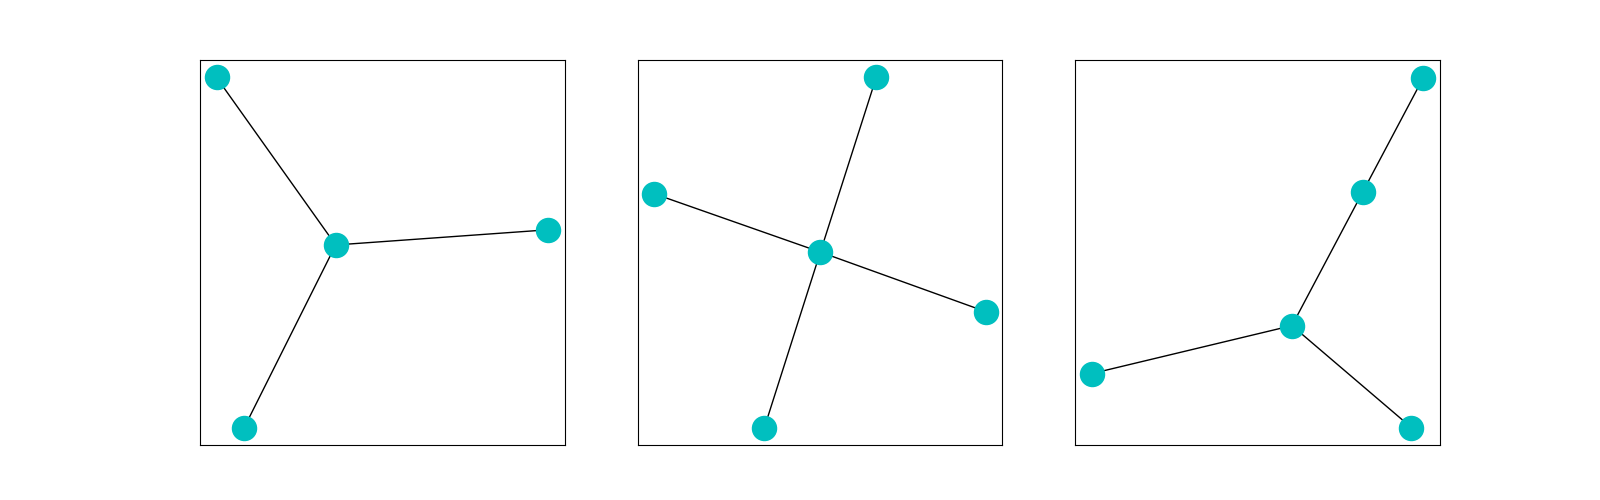
\includegraphics[width=14cm]{Images/H4_evolution.png}
    \centering
    \caption{The possible graphs generated by adding a node to the $H_{4}$ graph 
    and connecting it to an existing node.}
    \label{fig:H4T2}
\end{figure}

\begin{table}[h!]
    \centering
    \begin{tabular}{||c c c c||} 
    \hline
    Motif Count & Original Motif & Event 1 & Event 2\\ [0.5ex] 
    \hline\hline
    $H_{3}$ & 0 & 0 & 2\\ 
    \hline
    $H_{4}$ & 1 & 4 & 1\\
    \hline
    $H_{5}$ & 0 & 0 & 0\\
    \hline
   \end{tabular}
   \caption{Motif Counts of the $H_{4}$ motif and the possible 
   motifs given a $T2$ event.}
    \label{table:2}
\end{table}


\FloatBarrier


\section{The \texorpdfstring{$H_{5}$}{H5} Motif}
$H_{5}$'s are of interest due to the relationship they carry to the $H_{4}$, $H_{7}$, and $H_{8}$ motifs. The induced subgraph isomorphic to the $C_3$ in the motif, means we find two appearances of
$H_{5}$ in the $H_{7}$ and $H_{8}$ motifs. The $H_{4}$ is isomorphic to an induced subgraph of the $H_{5}$.The probabilities, given by 
 a preferential attachment mechanism, of the events
  in Figure ~\ref{fig:H5T2} the first event, $0.375$, for the second event, $0.125$, and the third event, $0.5$. The last event
only has the highest probability due to symmetry.

\begin{figure}[!ht]
    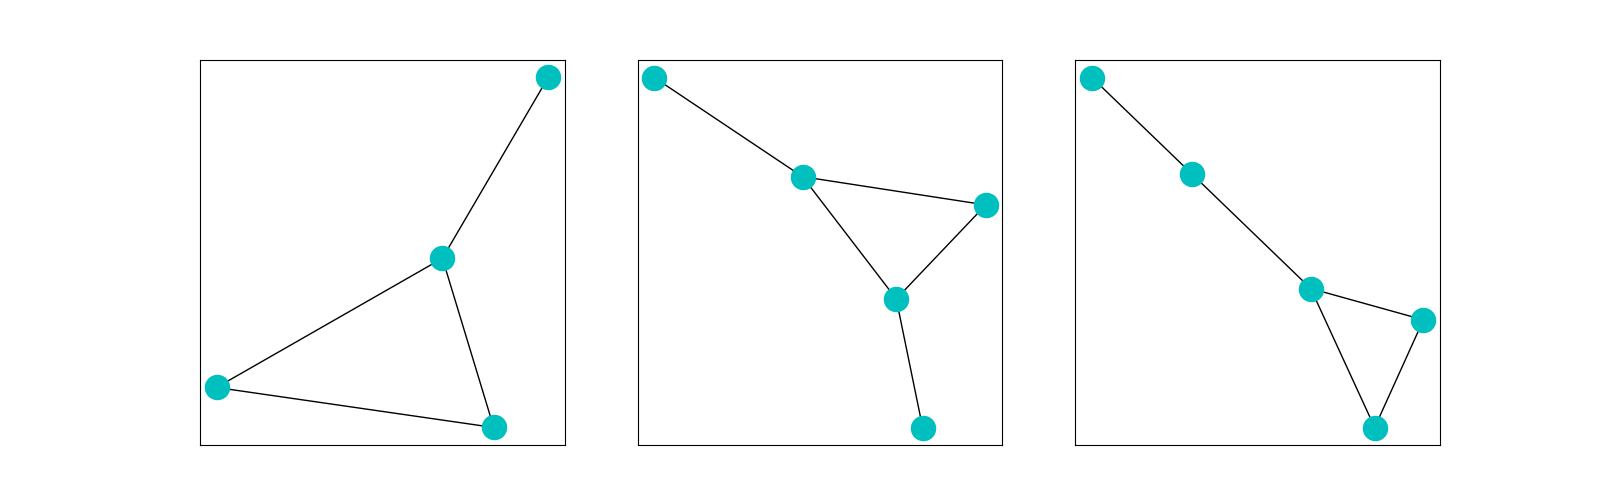
\includegraphics[width=12cm]{Images/H5_evolution.png}
    \centering
    \caption{The possible graphs generated by adding a node to the $H_{5}$ graph 
    and connecting it to an existing node}
    \label{fig:H5T2}
\end{figure}
\FloatBarrier

\begin{table}
    \centering
    \begin{tabular}{||c c c c c||} 
    \hline
    Motif Count & Original Motif & Event 1 & Event 2 & Event 3\\ [0.5ex] 
    \hline\hline
    $H_{3}$ & 2 & 4 & 4 & 5\\ 
    \hline
    $H_{4}$ & 1 & 4 & 1 & 2\\
    \hline
    $H_{5}$ & 1 & 2 & 1 & 2\\
    \hline
    $H_{6}$ & 0 & 0 & 0 & 0 \\
    \hline
    $H_{7}$ & 0 & 1 & 0 & 0 \\
    \hline
    $H_{8}$ & 0 & 0 & 0 & 1\\
    \hline
    $H_{9}$ & 0 & 0 & 1 & 0\\
    \hline
   \end{tabular}
   \caption{Motif counts of the possible $T2$ events on the $H_{5}$ motif.}
    \label{table:3}
\end{table}


\section{The \texorpdfstring{$H_{6}$}{H6} Motif}
The $H_{6}$ motif is formed by starting with an $H_{4}$ and adding two edges between the three outer nodes. It is 
almost a complete four-node graph. 
The $H_{6}$ motif count is not relatively high compared to other motifs in the Thij
model as it would require exact $T3$ events to generate them. Moreover, this
$T3$ event has to occur between what are likely non-root nodes. However, in the preferential attachment model for $m>2$
it is more likely to see many $H_{6}$ appearances because the preferential attachment model adds multiple edges from a single new node.

\begin{figure}[!ht]
    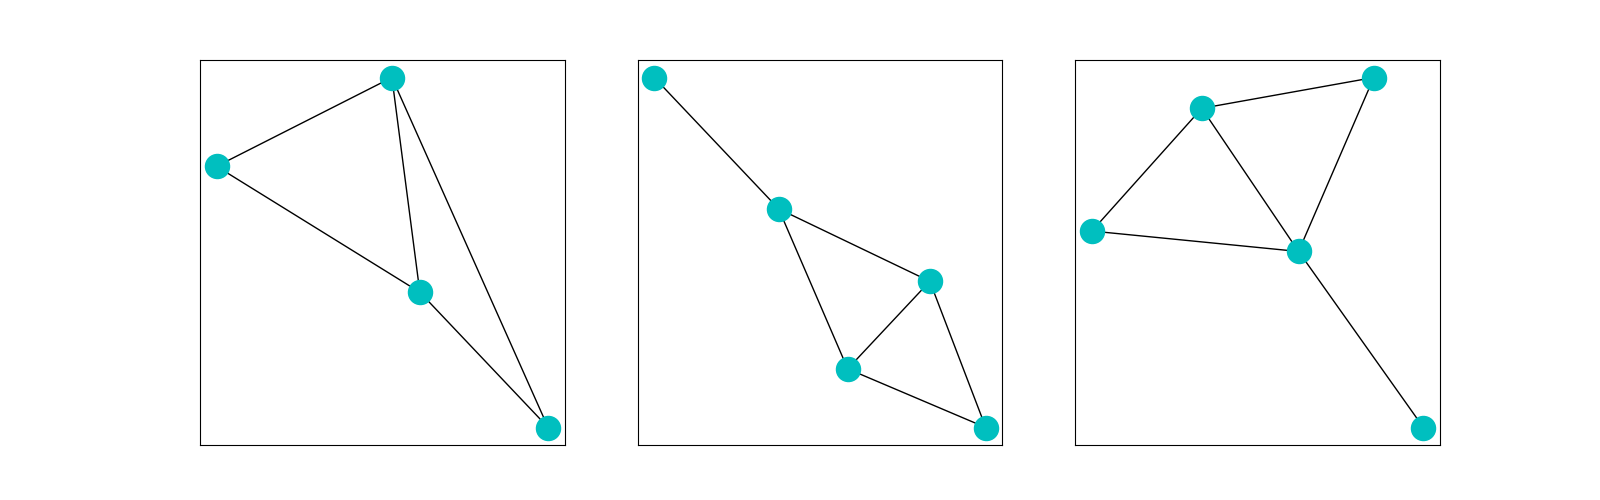
\includegraphics[width=14cm]{Images/H6_evolution.png}
    \centering
    \caption{The possible graphs generated by adding a node to the $H_{6}$ graph 
    and connecting it to an existing node}
\end{figure}
\FloatBarrier

\begin{table}
    \centering
    \begin{tabular}{||c c c c||} 
    \hline
    Motif Count & Original Motif & Event 1 & Event 2\\ [0.5ex] 
    \hline\hline
    $H_{3}$ & 6 & 10 & 10\\ 
    \hline
    $H_{4}$ & 2 & 3 & 5\\
    \hline
    $H_{5}$ & 4 & 5 & 6\\
    \hline
    $H_{6}$ & 1 & 1 & 1\\
    \hline
    $H_{7}$ & 0 & 0 & 2\\
    \hline
    $H_{8}$ & 0 & 2 & 2\\
    \hline
    $H_{9}$ & 0 & 1 & 1\\
    \hline
    $H_{10}$ & 0 & 2 & 0\\
    \hline
   \end{tabular}
   \caption{Motif counts for variations of the $T2$ event on the $H_{6}$ motif.}
    \label{table:4}
\end{table}

\section{The \texorpdfstring{$H_{7}$}{H7} Motif}
$H_{7}$ motifs feature prominently in the Thij model for $0<p \ll 1$. This is another consequence
of $S_k$ induced subgraphs in the networks. Connecting any two of the outer edges of $S_k$
will generate ${k-2 \choose 2}$ $H_{7}$ motifs. Assuming a graph has
formed with nodes attached to all three vertices of a $C_3$, the $H_{7}$ count is
the sum of ${d_i-2 \choose 2}$ for $i=1,2,3$ where $d_i$ is the degree of a single vertex of the $C_3$. We subtract 
2 from the degree $d_i$ recognizing the connections to the other vertices in the $C_3$ graph. Now for each vertex in the $C_3$
we can pick two attached nodes not in the $C_3$. These two connected nodes and the $C_3$ make up an appearance of $H7$. We count
these across all three nodes giving $\sum^{3}_{i=1}{d_i-2 \choose 2}$
  Adding a node to any one of those vertices $v_i$ in the $C_3$, assuming 
$d_i\geq 4$, will generate $d_i-2$ new $H_{7}$ appearances, a new appearance for each node connected to vertex $v_i$.

\begin{figure}[!ht]
    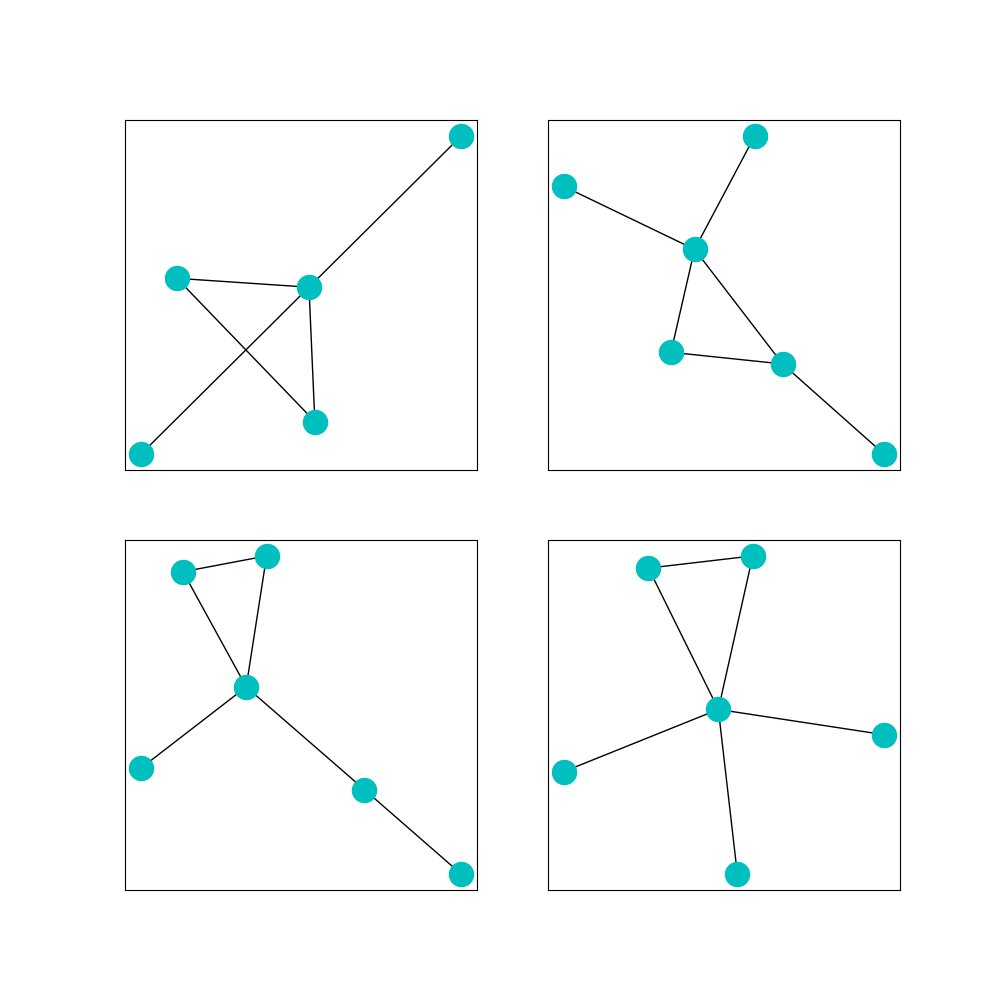
\includegraphics[width=12cm]{Images/H7_evolution.png}
    \centering
    \caption{The possible graphs generated by adding a node to the $H_{7}$ graph 
    and connecting it to an existing node}
\end{figure}
\FloatBarrier

\begin{table}
    \centering
    \begin{tabular}{||c c c c c||} 
    \hline
    Motif Count & Original Motif & Event 1 & Event 2 & Event 3 \\ [0.5ex] 
    \hline\hline
    $H_{3}$ & 4 & 8 & 7 & 6\\ 
    \hline
    $H_{4}$ & 4 & 5 & 4 & 10\\
    \hline
    $H_{5}$ & 2 & 3 & 2 & 3\\
    \hline
    $H_{6}$ & 0 & 0 & 0 & 0\\
    \hline
    $H_{7}$ & 1 & 1 & 1 & 3\\
    \hline
    $H_{8}$ & 0 & 2 & 0 & 0\\
    \hline
    $H_{9}$ & 0 & 0 & 0 & 0\\
    \hline
    $H_{10}$ & 0 & 0 & 1 & 0\\
    \hline
   \end{tabular}
   \caption{Motif counts of the $H_{7}$ motif and the possible additions of $T2$ event nodes.}
   \label{table:5}
\end{table}

\section{The \texorpdfstring{$H_{8}$}{H8} Motif}
The $H_{8}$ motif is another we expect to appear fairly often. The $H_{8}$
is two $H_{4}$'s sharing an edge and a node. We can also characterize
it as a $C_3$ graph with two nodes attached to distinct vertices on the $C_3$. Given a $C_3$ graph with at-least one node attached
to each vertex, we have $(d_i-2)(d_j-2)(d_k-2)$ $H_{8}'s$. The number of new 
$H_{8}$'s by connecting a node to vertex $v_i$ is given by $(d_j-2)(d_k-2)$.

\begin{figure}[!ht]
    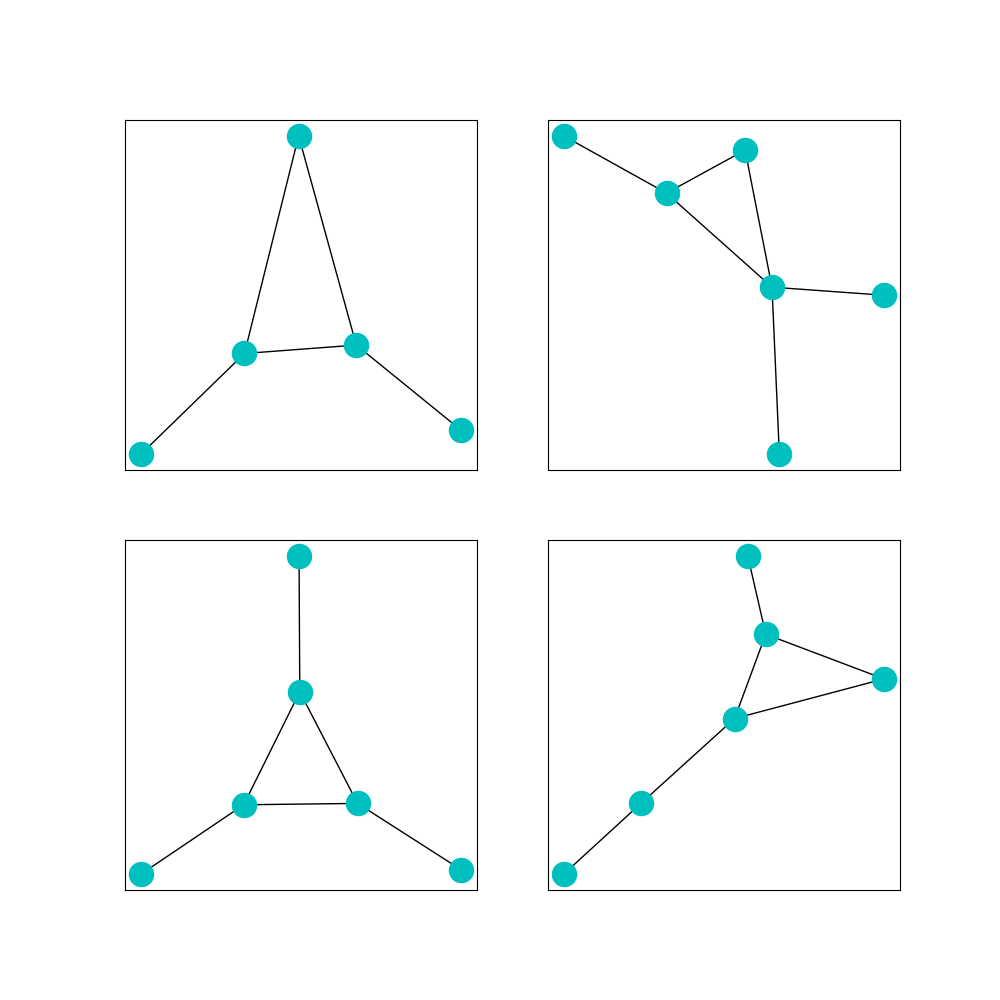
\includegraphics[width=12cm]{Images/H8_evolution.png}
    \centering
    \caption{The possible graphs generated by adding a node to the $H_{8}$ graph 
    and connecting it to an existing node}
\end{figure}

\FloatBarrier
\begin{table}
    \centering
    \begin{tabular}{||c c c c c||} 
    \hline
    Motif Count & Original Motif & Event 1 & Event 2 & Event 3 \\ [0.5ex] 
    \hline\hline
    $H_{3}$ & 5 & 8 & 9 & 7\\ 
    \hline
    $H_{4}$ & 2 & 5 & 3 & 2 \\
    \hline
    $H_{5}$ & 2 & 3 & 3 & 2 \\
    \hline
    $H_{6}$ & 0 & 0 & 0 & 0 \\
    \hline
    $H_{7}$ & 0 & 1 & 0 & 0 \\
    \hline
    $H_{8}$ & 1 & 2 & 3 & 1\\
    \hline
    $H_{9}$ & 0 & 0 & 0 & 0\\
    \hline
    $H_{10}$ & 0 & 0 & 0 & 1\\
    \hline
   \end{tabular}
   \caption{Motif counts graphs formed by possible $T2$ events on the $H_{8}$ motif.}
   \label{table:6}
\end{table}

\section{ The \texorpdfstring{$H_{9}$}{H9} motif}
The $H_{9}$ motif appearances do not form around stars in the same way we might expect $H_{7}$ and $H_{8}$ appearances.
 The $H_{9}$ motif could develop in a way similar to the $H_{5}$. This is because the $H_{9}$ has an induced subgraph
 isomorphic to the $C_4$. The $H_{9}$ is produced by attaching a node to any one of those vertices in the induced
 subgraph. Given a $C_4$ and attachment
 of new nodes to any of its four vertices, the count of $H_{9}$'s is simply the sum of the degrees of each
 vertex minus 2. The growth is additive, not combinatorial in the manner of $H_{7}$'s or $H_{8}$'s.

\begin{figure}[!ht]
    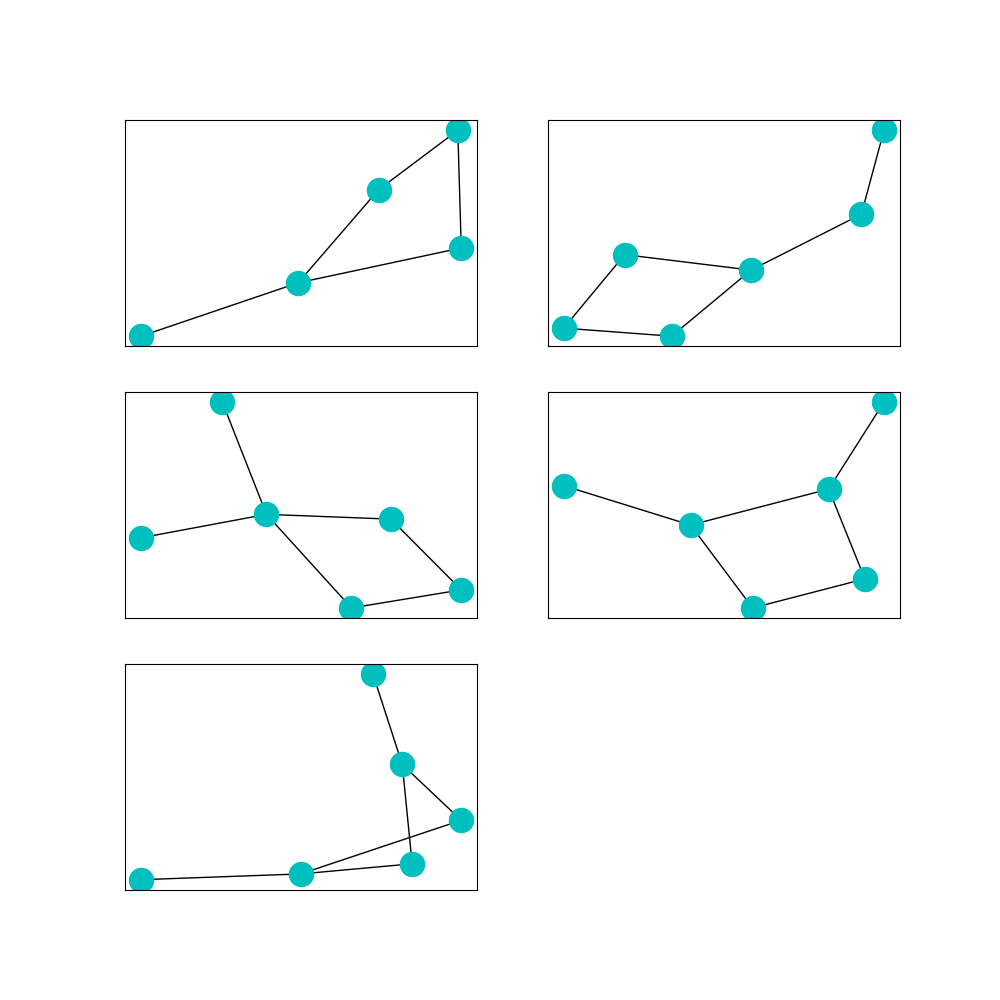
\includegraphics[width=12cm]{Images/H9_evolution.png}
    \centering
    \caption{The possible graphs generated by adding a node to the $H_{9}$ graph 
    and connecting it to an existing node}
\end{figure}

\begin{table}
    \centering
    \begin{tabular}{||c c c c c c ||} 
    \hline
    Motif Count & Original Motif & Event 1 & Event 2 & Event 3  & Event 4\\ [0.5ex] 
    \hline\hline
    $H_{3}$ & 6 & 8 & 8 & 9 & 8\\ 
    \hline
    $H_{4}$ & 1 & 1 & 4 & 2 & 2 \\
    \hline
    $H_{5}$ & 0 & 0 & 0 & 0 & 0\\
    \hline
    $H_{6}$ & 0 & 0 & 0 & 0 & 0\\
    \hline
    $H_{7}$ & 0 & 0 & 0 & 0 & 0\\
    \hline
    $H_{8}$ & 0 & 0 & 0 & 0& 0\\
    \hline
    $H_{9}$ & 1 & 1 & 2 & 2 &2\\
    \hline
   \end{tabular}
   \caption{Motif counts graphs formed by possible $T2$ events on the $H_{9}$ motif.}
   \label{table:7}
\end{table}

\section{The \texorpdfstring{$H_{10}$}{H10} Motif}
The $H_{10}$ motif graph is a $H_{9}$ graph with an extra vertex. There is an edge connecting that vertex to the 
single vertex of degree one in the $H_{9}$ graph. Many $H_{10}$ appearances could be generated from a single $H_{9}$ if vertices
attach to the single vertex of degree one in the $H_{9}$ motif. A star graph would form
with that vertex at the center. The growth for the $H_{10}$ in the preferential mechanism with $k=1$ is additive.
For $k>1$, it is possible clusters of triangles could form causing the $H_{10}$ motif count to increase faster than by the addition of a single node and edge at each time-step. 

\begin{figure}[!ht]
    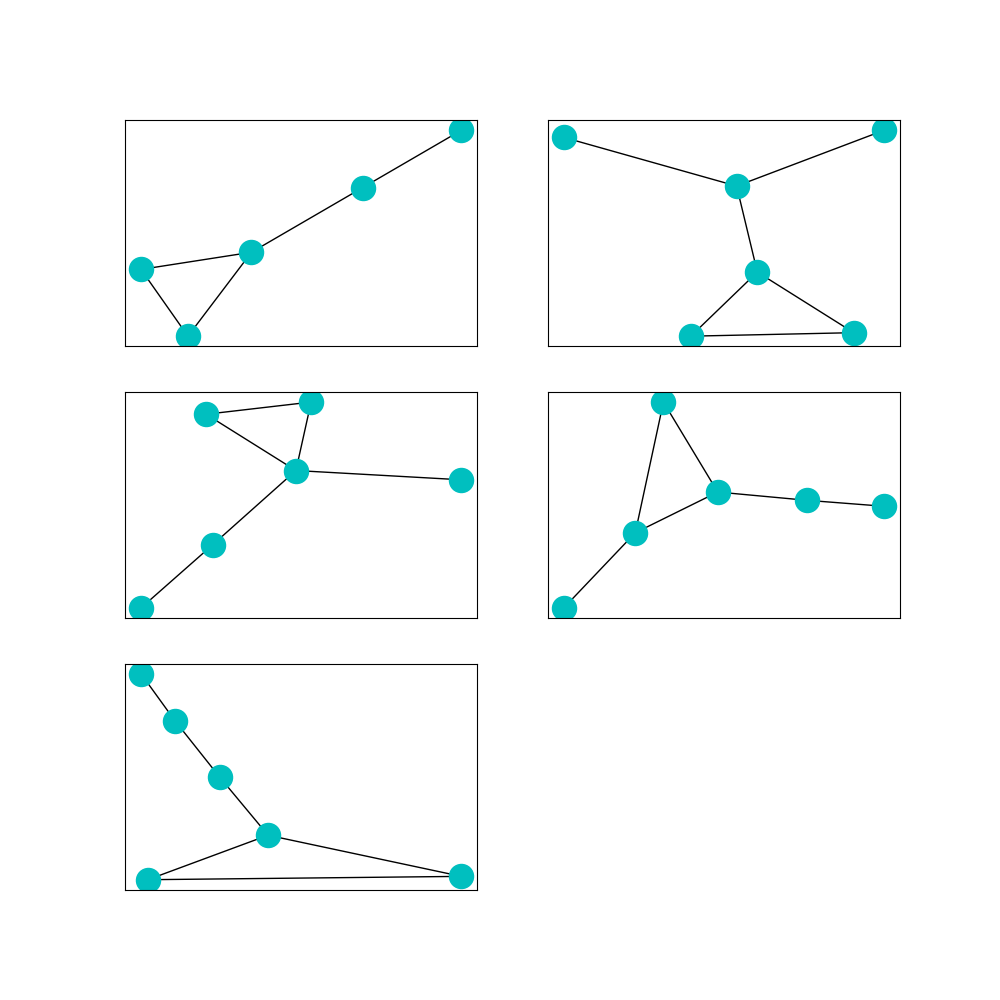
\includegraphics[width=12cm]{Images/H10_evolution.png}
    \centering
    \caption{The possible graphs generated by adding a node to the $H_{10}$ graph 
    and attaching it to an existing node.}
\end{figure}

\begin{table}
    \centering
    \begin{tabular}{||c c c c c c ||} 
    \hline
    Motif Count & Original Motif & Event 1 & Event 2 & Event 3  & Event 4 \\ [0.5ex] 
    \hline\hline
    $H_{3}$ & 4 & 6 & 7 & 7  & 5\\
    \hline
    $H_{4}$ & 1 & 2 & 4 & 2  & 1\\
    \hline
    $H_{5}$ & 1 & 1 & 2 & 2 & 1\\
    \hline
    $H_{6}$ & 0 & 0 & 0 & 0  & 5\\
    \hline
    $H_{7}$ & 0 & 0 & 1 & 0 & 0 \\
    \hline
    $H_{8}$ & 0 & 0 & 0 & 1 & 0 \\
    \hline
    $H_{9}$ & 0 & 0 & 0 & 0  & 0 \\
    \hline
    $H_{10}$ & 1 & 2 & 1 & 1 & 1 \\
    \hline
   \end{tabular}
   \caption{Motifs counts of the possible $T2$ event on the $H_{10}$ motif.}
   \label{table:8}
\end{table}

\FloatBarrier

\section{The \texorpdfstring{$H_{11}$}{H11} Motif}
The $H_{11}$ motif, shaped like a bow-tie, is formed by two three-walks that share a common
vertex. This motif does need $k \geq 2$ in the Barabási–Albert Model or
 a $T3$ event to form an edge between two existing nodes. The $H_{11}$ motif does not appear 
 commonly without those necessary criteria.

\begin{figure}[!ht]
    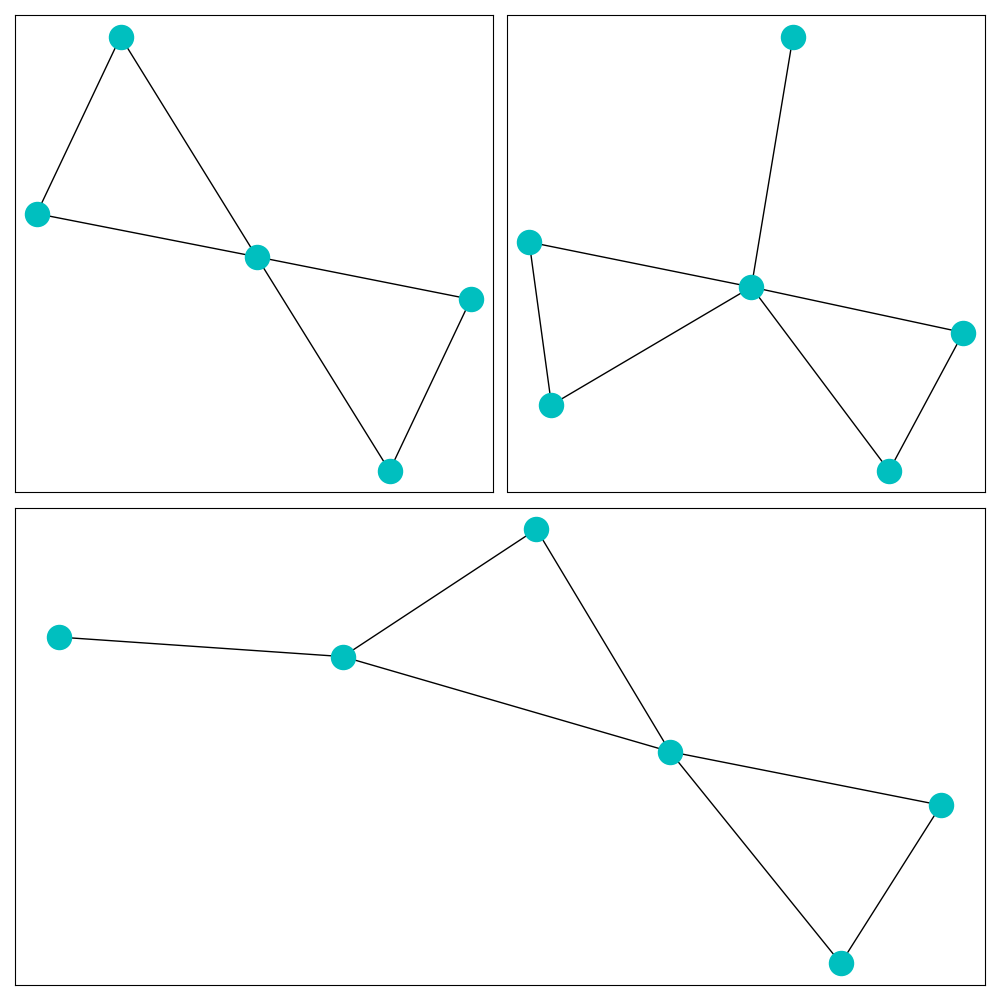
\includegraphics[width=8cm]{Images/H11_evolution.png}
    \centering
    \caption{The possible graphs generated by adding a node to the $H_{11}$ graph 
    and connecting it to an existing node.}
\end{figure}

\begin{table}
    \centering
    \begin{tabular}{||c c c c||} 
    \hline
    Motif Count & Original Motif & Event 1 & Event 2 \\ [0.5ex] 
    \hline\hline
    $H_{3}$ & 8 & 12 & 12 \\ 
    \hline
    $H_{4}$ & 4 & 5 & 10  \\
    \hline
    $H_{5}$ & 0 & 5 & 6  \\
    \hline
    $H_{6}$ & 0 & 0 & 0  \\
    \hline
    $H_{7}$ & 2 & 2 & 6 \\
    \hline
    $H_{8}$ & 0 & 2 & 0 \\
    \hline
    $H_{9}$ & 0 & 0 & 0 \\
    \hline
    $H_{10}$ & 4 & 5 & 4 \\
    \hline
    $H_{11}$ & 1 & 1 & 1\\
    \hline
   \end{tabular}
   \caption{Motif counts of the graphs generated by possible $T2$ events on the $H_{11}$ motif.}
   \label{table:9}
\end{table}

\FloatBarrier

\section{The \texorpdfstring{$H_{12}$}{H12} Motif}
$H_{12}$, shaped like a house, contains five nodes, six edges, with an induced subgraph isomorphic to $C_4$
and a single vertex attached to two vertices themselves connected. The $H_{12}$, like other
motifs, containing an induced subgraph isomorphic to $C_4$, is not a priori expected to have a relatively large count
given the preferential attachment mechanism. 

\begin{figure}[!ht]
    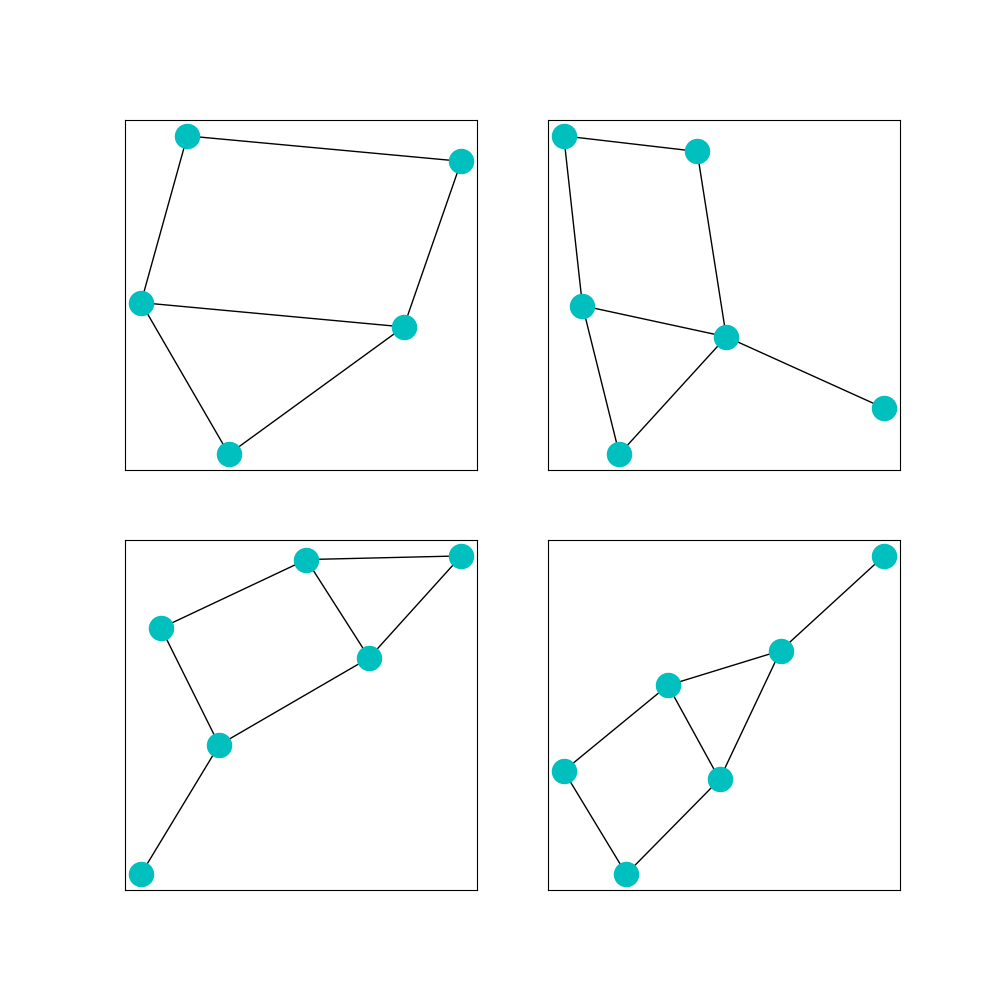
\includegraphics[width=12cm]{Images/H12_evolution.png}
    \centering
    \caption{The possible graphs generated by adding a node to the $H_{12}$ graph 
    and connecting it to an existing node.}
\end{figure}

\begin{table}
    \centering
    \begin{tabular}{||c c c c c||} 
    \hline
    Motif Count & Original Motif & Event 1 & Event 2 & Event 3 \\ [0.5ex] 
    \hline\hline
    $H_{3}$ & 10 & 14 & 13 & 14\\ 
    \hline
    $H_{4}$ & 2 & 5 & 3 & 3 \\
    \hline
    $H_{5}$ & 2 & 3 & 2 & 3 \\
    \hline
    $H_{6}$ & 0 & 0 & 0 & 0 \\
    \hline
    $H_{7}$ & 0 & 1 & 0 & 0 \\
    \hline
    $H_{8}$ & 1 & 2 & 1 & 3\\
    \hline
    $H_{9}$ & 2 & 3 & 3 & 2 \\
    \hline
    $H_{10}$ & 2 & 2 & 3 & 2 \\
    \hline
    $H_{11}$ & 0 & 0 & 0 & 0 \\
    \hline
    $H_{12}$ & 1 & 1 & 1 & 1\\
    \hline
   \end{tabular}
   \caption{Variations of the $T2$ event on the $H_{12}$ motif}
   \label{table:10}
\end{table}


\FloatBarrier

\section{The \texorpdfstring{$H_{13}$}{H3} Motif}
The $H_{13}$ could plausibly form in the $k \geq 2$ case for the 
Barabási–Albert model, but it would require a new node consistently attached correctly to an $H_{6}$ appearance.
 For this process of generating new $H_{13}$'s, the increase in the motif counts is additive.
 Thus for the Barabási–Albert model of $0<k<3$, the presence of an $H_{13}$ is sensitive
to the initial graph.

\begin{figure}[!ht]
    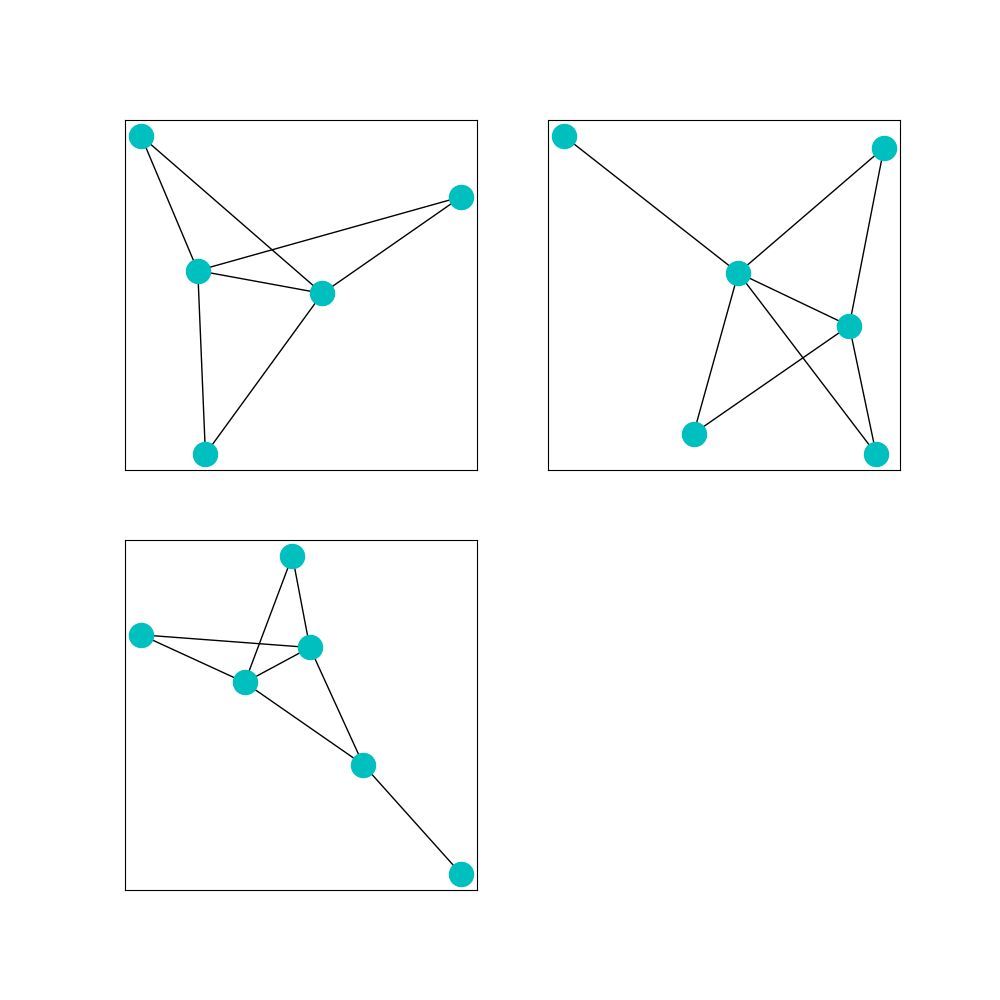
\includegraphics[width=8cm]{Images/H13_evolution.png}
    \centering
    \caption{The $H_{13}$ graph and possible node attachments up to symmetry.}
\end{figure}

\begin{table}
    \centering
    \begin{tabular}{||c c c c||} 
    \hline
    Motif Count & Original Motif & Event 1 & Event 2 \\ [0.5ex] 
    \hline\hline
    $H_{3}$ & 18 & 24 & 24\\ 
    \hline
    $H_{4}$ & 8 & 14 & 9  \\
    \hline
    $H_{5}$ & 12 & 15 & 13  \\
    \hline
    $H_{6}$ & 3 & 3 &3  \\
    \hline
    $H_{7}$ & 6 & 12 & 6 \\
    \hline
    $H_{8}$ & 6 & 12 & 10\\
    \hline
    $H_{9}$ & 6 & 9 & 8 \\
    \hline
    $H_{10}$ & 0 & 0 & 4  \\
    \hline
    $H_{11}$ & 0 & 0 & 0  \\
    \hline
    $H_{12}$ & 0 & 0 & 0 \\
    \hline
    $H_{13}$ & 1 & 1 & 1 \\
    \hline
   \end{tabular}
   \caption{Motif counts of the possible $T2$ events on the $H_{13}$ motif}
   \label{table:11}
\end{table}

\section{Summary of Preferential Attachment and \texorpdfstring{$T2$}{T2} Event Motif Evolution}


Motif development in the Barabási–Albert model is dependent on the initialization of nodes and 
the choice of $k$. Adding $k=1$ edges for every new node
 limits the motifs that can appear. There will be no new $H_{6}$, $H_{11}$,
$H_{12}$, or $H_{13}$ appearances generated. There is no possible way for them to form as there is no
node of degree one in those motif graphs. Only upon taking $k>1$ could those motif counts change over
 time. Some graphs are more likely to have a high number of appearances for $k=2$ than others, like the $H_{4}$, $H_{7}$, and $H_{8}$ motifs.

This analysis also applies to the $T2$ event in the Thij model. The occurrence is similar to
the preferential attachment model with $k=1$ as it is the addition of a node 
connected to a single existing node. The $T2$ event, unlike the BA model, selects a message tree 
and then uses a superstar attachment mechanism to attach to a node with probability $q=0.9$. Even when the network is relatively
small, nodes will still overwhelmingly attach to the root message node. This mechanism is
much more likely to generate $H_{4}$'s, as seen in Chapter 3. If the root
message node is the vertex of a $C_3$ isomorphic subgraph, then we may see $H_{7}$ and $H_{8}$ counts
rapidly increase over time, correlating with the $H_{4}$ count. 

\section{Twitter Model Specific Motif Evolution}

In Chapter 3, we specified three possible
events in the Thij model: a new root node, a new node with an attached edge, or a new edge between existing nodes 
($T1$, $T2$, $T3$ respectively). The only events specific to the Thij model are $T1$ and $T3$ events. 
$T1$ events add a new message node, but they do not immediately affect any change in the motif counts.
They could potentially have an impact on motif enumeration with the right $T3$ event or a sequence of $T2$ events.
 The $T3$ event we briefly consider because a $T3$ event can change the composition of the network in ways $T2$ events cannot.

The $T3$ event is a much more complex mechanism than the $T2$ event. 
$T3$'s can add edges \textit{between} different motif graphs and to a single motif's graph. If two motifs
are disjoint, a $T3$ event bridges them and acts as multiple $T2$ events on both motifs. This is still a simple case,
 but for the eleven non-simple cycle motifs considered there are 55 different possibilities of inter-motif
 interaction. If the $T3$ event bridges two large disjoint graphs, this could affect many different motif appearances simultaneously. 

The $T3$ event opens up new possibilities for the model. $C_3$ and $C_4$ appearances
are more likely to form around root nodes. A $T2$ event alone cannot generate new $C_3$ or $C_4$ appearances. We may see more 
$H_{6}$ up to $H_{13}$ appearances because they require $C_3$ and $C_4$ appearances in the network in order to form.
 For $p=0.2$, the Thij model exhibits significantly more clustering throughout time because of this $T3$ attachment mechanism.
  Measuring the impact of a small $p$ parameter
  is for the tools of statistical analysis because there are too many cases to consider by graphical analysis. 


% \section{H_{3}}
% The $H_{3}$ motif only has two possible events. We see either an $H_{5}$ form by connecting
% an outer vertex to the opposite inner or the outer two vertices are connected
% forming a four-cycle. Future development of this new $H_{5}$ in the context of 
% $T3$ events is discussed in section 6.3. 

% \begin{figure}[!ht]
%     \includegraphics[width=15cm]{Images/H_{3}_T3_evolution.png}
%     \centering
%     \caption{The possible graphs generated by adding an edge to the $H_{3}$ graph.}
% \end{figure}

% \begin{table}
%     \centering
%     \begin{tabular}{||c c c c||} 
%     \hline
%     Motif Count & Original Motif & Event 1 & Event 2\\ [0.5ex] 
%     \hline\hline
%     H_{3} & 1 & 2 & 4\\ 
%     \hline
%     H_{4} & 0& 1 & 0  \\
%     \hline
%     H_{5} & 0& 1 & 0  \\
%     \hline
%    \end{tabular}
%    \caption{Motif counts of the possible $T3$ events on the $H_{3}$ motif}
%    \label{table:12}
% \end{table}

% \section{H_{4}}
% Due to the three symmetry of the $H_{4}$, adding an edge between any two unconnected nodes creates a single $H_{5}$. Therefore given some balance between $T2$ and $T3$ events
% we could see correlation between these two motifs.

% \begin{figure}[!ht]
%     \includegraphics[width=14cm]{Images/H_{4}_T3_evolution.png}
%     \centering
%     \caption{The possible graphs generated by adding an edge to the $H_{4}$ graph. By connecting the 
%     two outer edges we find a $C_4$ and by connecting an outer vertex to an inner vertex we generate a $H_{5}$.}
% \end{figure}

% \begin{table}
%     \centering
%     \begin{tabular}{||c c c||} 
%     \hline
%     Motif Count & Original Motif & Event 1 \\ [0.5ex] 
%     \hline
%     H_{3} & 0 & 2 \\ 
%     \hline
%     H_{4} & 1 & 1 \\
%     \hline
%     H_{5} & 0 & 1 \\
%     \hline
%    \end{tabular}
%    \caption{Motif counts of the $T3$ event on the $H_{4}$ motif}
%    \label{table:13}
% \end{table}

% \section{H_{5}}
% The $H_{5}$ motif is symmetric. Connecting any two unconnected vertices of the $H_{5}$ produces a $H_{6}$.
% A $H_{4}$ with a $T3$ event creates a $H_{5}$ graph. A $T3$ event occurs again on the same graph and a $H_{6}$
% graph is produced.

% \begin{figure}[!ht]
%     \includegraphics[width=14cm]{Images/H_{5}_T3_evolution.png}
%     \centering
%     \caption{The possible graphs generated by adding an edge to the $H_{5}$ graph.}
% \end{figure}

% \begin{table}
%     \centering
%     \begin{tabular}{||c c c||} 
%     \hline
%     Motif Count & Original Motif & Event 1 \\ [0.5ex] 
%     \hline\hline
%     H_{3} & 2 & 6\\ 
%     \hline
%     H_{4} & 1 & 2 \\
%     \hline
%     H_{5} & 1 & 4\\
%     \hline
%     H_{6} & 0 & 1\\
%     \hline
%    \end{tabular}
%    \caption{Motif counts of the graphs produced by a $T3$ event on the $H_{5}$ motif.}
%    \label{table:14}
% \end{table}

% \section{H_{6}}
% Adding an edge to $H_{6}$ generates a complete graph of four nodes. This 
% event is unlikely given a large graph, but not impossible. If a vertex
% of the $H_{6}$ is a message node then an edge could be added within the $H_{6}$ graph. 
% However, an edge added between the $H_{6}$ appearance and the appearance of another 
% motif is more likely. 

% \begin{figure}[!ht]
%     \includegraphics[width=14cm]{Images/H_{6}_T3_evolution.png}
%     \centering
%     \caption{The possible graphs generated by adding an edge to the $H_{6}$ graph.}
% \end{figure}

% \begin{table}
%     \centering
%     \begin{tabular}{||c c c ||} 
%     \hline
%     Motif Count & Original Motif & Event 1  \\ [0.5ex] 
%     \hline\hline
%     H_{3} & 6 & 12 \\ 
%     \hline
%     H_{4} & 2 & 4 \\
%     \hline
%     H_{5} & 4 & 12 \\
%     \hline
%     H_{6} & 1 & 6 \\
%     \hline
%     \hline
%    \end{tabular}
%    \caption{Motif counts of graph produced by a $T3$ event on the $H_{6}$ motif.}
% \end{table}

% \section{H_{7}}
% Adding edges, the $H_{7}$ motif gives only two non-isomorphic graphs as 
% a consequence of the motif's symmetry. Given an event two in figure ~\ref{fig:H_{7}T3} the graph becomes
% an $H_{11}$. Both events do show that one could see a high $H_{7}$ count given enough
% clustering around a message node. 
 
% \begin{figure}[!ht]
%     \includegraphics[width=16cm]{Images/H_{7}_T3_evolution.png}
%     \centering
%     \caption{The possible graphs generated by adding an edge to the $H_{7}$ graph.}
%     \label{fig:H_{7}T3}
% \end{figure}

% \begin{table}
%     \centering
%     \begin{tabular}{||c c c c||} 
%     \hline
%     Motif Count & Original Motif & Event 1 & Event 2  \\ [0.5ex] 
%     \hline\hline
%     H_{3} & 4 & 10 & 8\\ 
%     \hline
%     H_{4} & 4 & 5& 4 \\
%     \hline
%     H_{5} & 2 & 6 & 4 \\
%     \hline
%     H_{6} & 0 & 1 & 0 \\
%     \hline
%     H_{7} & 1 & 2 & 2 \\
%     \hline
%     H_{8} & 0 & 2 & 0\\
%     \hline
%     H_{9} & 0 & 1 & 0 \\
%     \hline
%     H_{10} & 0 & 0 & 4 \\
%     \hline
%     H_{11} & 0 & 0 & 1\\
%     \hline
%    \end{tabular}
%    \caption{Motif counts of the two possible graphs produced by the $T3$ event on the $H_{7}$ motif}
%    \label{table:16}
% \end{table}

% \section{H_{8}}
% The $H_{8}$ motif here generates three different motifs depending upon the nodes which become connected.
% The $H_{8}$ motif is similar to the $H_{7}$ motif as clusters of triangles can contain many $H_{8}$ appearances. 

% \begin{figure}[!ht]
%     \includegraphics[width=12cm]{Images/H_{8}_T3_evolution.png}
%     \centering
%     \caption{The possible graphs generated by adding an edge to the $H_{8}$ graph.}
% \end{figure}

% \begin{table}
%     \centering
%     \begin{tabular}{||c c c c c||} 
%     \hline
%     Motif Count & Original Motif & Event 1 & Event 2 & Event 3 \\ [0.5ex] 
%     \hline\hline
%     H_{3} & 5 & 10 & 10 & 10\\ 
%     \hline
%     H_{4} & 2 & 5 & 3 & 2 \\
%     \hline
%     H_{5} & 2 & 6 & 5 & 2 \\
%     \hline
%     H_{6} & 0 & 1 & 1 & 0 \\
%     \hline
%     H_{7} & 0 & 2 & 0 & 0 \\
%     \hline
%     H_{8} & 1 & 2 & 2 & 1\\
%     \hline
%     H_{9} & 0 & 1 & 1 & 2\\
%     \hline
%     H_{10}  & 0 & 0 & 2& 2 \\
%     \hline
%     H_{11}  & 0 & 0 & 1& 0 \\
%     \hline
%     H_{12}  & 0 & 0 & 0& 0 \\
%     \hline
%    \end{tabular}
%    \caption{Motif counts of the possible $T3$ event on the $H_{8}$ motif}
%    \label{table:17}
% \end{table}

% \section{H_{9}}
% An $H_{9}$ motif with an edge added anywhere does not produce a combinatorial jump in counts as
%  other motifs might. The $H_{9}$ had an induced subgraph, isomorphic to the $C_4$ which
%  means the graph requires more events or the right initialization to generate more $H_{9}$. Given
%  a high $T3$ probability, there are relatively high $H_{9}$ counts as seen in figures ~\ref{fig:pthij0202}
% and ~\ref{fig:pthij0802}.

% \begin{figure}
%     \includegraphics[width=14cm]{Images/H_{9}_T3_evolution.png}
%     \centering
%     \caption{The possible graphs generated by adding an edge to the $H_{9}$ graph.}
% \end{figure}

% \begin{table}
%     \centering
%     \begin{tabular}{||c c c c c c||} 
%     \hline
%     Motif Count & Original Motif & Event 1 & Event 2 & Event 3 & Event 4 \\ [0.5ex] 
%     \hline\hline
%     H_{3} & 6 & 10 & 10 & 10 & 10\\ 
%     \hline
%     H_{4} & 1 & 5 & 3 & 2 & 2 \\
%     \hline
%     H_{5} & 0 & 6 & 5 & 2 & 2 \\
%     \hline
%     H_{6} & 0 & 1 & 1 & 0 & 0 \\
%     \hline
%     H_{7} & 1 & 2 & 1 & 0 & 0 \\
%     \hline
%     H_{8} & 0 & 2 & 2 & 1 & 1\\
%     \hline
%     H_{9} & 1 & 1 & 2 & 2 & 2\\
%     \hline
%     H_{10} & 0 & 0 & 2 & 2 & 2\\
%     \hline
%     H_{11} & 0 & 0 & 0 & 0 & 0\\
%     \hline
%     H_{12} & 0 & 0 & 0 & 1 & 1\\
%     \hline
%    \end{tabular}
%    \caption{Motif counts of the possible $T3$ event on the $H_{9}$ motif}
%    \label{table:18}
% \end{table}

% \section{H_{10}}
% The $H_{10}$ motif features in those Thij models with $p<0.5$ line in figures ~\ref{fig:pthij0202} and
% ~\ref{fig:pthij0808}, given
% that there is enough likelihood a $T3$ event occurs acting on an $H_{9}$. For events two, three, and four below
% in Figure~\ref{fig:H_{10}T3}, attaching a node to the $H_{10}$ motif produces a handful more of $H_{10}$'s.


% \begin{figure}
%     \includegraphics[width=12cm]{Images/H_{10}_T3_evolution.png}
%     \centering
%     \caption{The possible graphs generated by adding an edge to the $H_{10}$ graph.}
%     \label{fig:H_{10}T3}
% \end{figure}

% \begin{table}
%     \centering
%     \begin{tabular}{||c c c c c||} 
%     \hline
%     Motif Count & Original Motif & Event 1 & Event 2 & Event 3 \\ [0.5ex] 
%     \hline\hline
%     H_{3} & 4 & 10 & 8 & 10 \\ 
%     \hline
%     H_{4} & 1 & 2 & 4 & 3 \\
%     \hline
%     H_{5} & 1 & 2 & 4 & 5\\
%     \hline
%     H_{6} & 0 & 0 & 0 & 1 \\
%     \hline
%     H_{7} & 0 & 0 & 2 & 0 \\
%     \hline
%     H_{8} & 0 & 1 & 0 & 2\\
%     \hline
%     H_{9} & 0 & 2 & 0 & 1\\
%     \hline
%     H_{10} & 1 & 2 & 4 & 2\\
%     \hline
%     H_{11} & 0 & 0 & 1 & 0\\
%     \hline
%     H_{12} & 0 & 1 & 0 & 0\\
%     \hline
%    \end{tabular}
%    \caption{Motif counts of the graphs given by a $T3$ event on the $H_{10}$ motif}
%    \label{table:19}
% \end{table}

% \section{H_{11}}
% $H_{11}$'s do not appear prominently in any of the simulations because they are isomorphic to
% two $C_3$'s connect at a single vertex. To produce an $H_{11}$ from an existing $H_{11}$ appearance,
% one would need to connect both vertices of a two-walk to a $H_{11}$ vertex.

% \begin{figure}
%     \includegraphics[width=12cm]{Images/H_{11}_T3_evolution.png}
%     \centering
%     \caption{The possible graphs generated by adding an edge to the $H_{11}$ graph.}
% \end{figure}

% \begin{table}
%     \centering
%     \begin{tabular}{||c c c ||} 
%     \hline
%     Motif Count & Original Motif & Event 1 \\ [0.5ex] 
%     \hline\hline
%     H_{3} & 8 & 17 \\ 
%     \hline
%     H_{4} & 4 & 6  \\
%     \hline
%     H_{5} & 4 & 10 \\
%     \hline
%     H_{6} & 0 & 2 \\
%     \hline
%     H_{7} & 2 & 3 \\
%     \hline
%     H_{8} & 0 & 5 \\
%     \hline
%     H_{9} & 0 & 4 \\
%     \hline
%     H_{10} & 4 & 6 \\
%     \hline
%     H_{11} & 1 & 1 \\
%     \hline
%     H_{12} & 0 & 2 \\
%     \hline
%     H_{13} & 0 & 0 \\
%     \hline
%    \end{tabular}
%    \caption{Motif counts of the single graph produced by a $T3$ event on the $H_{11}$ motif}
%    \label{table:20}
% \end{table}

% \section{H_{12}}
% As we discussed in section 5.10, the $H_{12}$ motifs are not commonly found in the network simulations
% because they require a four-walk. In the Thij model, assuming the presence of an $H_{12}$,
% one could generate more $H_{12}$'s by a $T2$ event to a vertex of the four-cycle and then a 
% $T3$ event to follow. In table ~\ref{table:H_{13}T3} we see even a single $T3$ would suffice to produce two or even four new
% $H_{12}$'s.

% \begin{figure}
%     \includegraphics[width=12cm]{Images/H_{12}_T3_evolution.png}
%     \centering
%     \caption{The possible graphs generated by adding an edge to the $H_{12}$ graph.}
% \end{figure}

% \begin{table}
%     \centering
%     \begin{tabular}{||c c c c||} 
%     \hline
%     Motif Count & Original Motif & Event 1 & Event 2\\ [0.5ex] 
%     \hline\hline
%     H_{3} & 10 & 17 & 18 \\ 
%     \hline
%     H_{4} & 2 & 6 & 4 \\
%     \hline
%     H_{5} & 2 & 10 & 6\\
%     \hline
%     H_{6} & 0 & 2 & 1 \\
%     \hline
%     H_{7} & 0 & 3 & 0\\
%     \hline
%     H_{8} & 1 & 5 & 4 \\
%     \hline
%     H_{9} & 2 & 4 & 8 \\
%     \hline
%     H_{10} & 2 & 6 & 6 \\
%     \hline
%     H_{11} & 0 & 1 & 0 \\
%     \hline
%     H_{12} & 1 & 2 & 4 \\
%     \hline
%     H_{13} & 0 & 0 & 0\\
%     \hline
%    \end{tabular}
%    \caption{Motif counts of the possible $T3$ event on the $H_{12}$ motif.}
%    \label{table:H_{13}T3}
% \end{table}

% \section{H_{13}}
% The $H_{13}$ does not frequently appear in any of the simulations. $H_{13}$ appearances
% are not readily generated from an existing $H_{13}$ appearances. To generate new appearances,
% one requires exact $T2$ and $T3$ events. Contrast this to an $H_{7}$
% or an $H_{8}$ which upon a $T3$ event alone can generate new $H_{7}$ or $H_{8}$ appearances. The $H_{13}$
% requires events to occur, which are not likely given the attachment mechanism. 

% \begin{figure}
%     \includegraphics[width=12cm]{Images/H_{13}_T3_evolution.png}
%     \centering
%     \caption{The possible graph generated by a $T3$ event on the $H_{13}$.}
% \end{figure}

% \begin{table}
%     \centering
%     \begin{tabular}{||c c c||} 
%     \hline
%     Motif Count & Original Motif & Event 1\\ [0.5ex] 
%     \hline\hline
%     H_{3} & 18 & 28 \\ 
%     \hline
%     H_{4} & 8 & 10 \\
%     \hline
%     H_{5} & 12 & 22 \\
%     \hline
%     H_{6} & 3 & 8 \\
%     \hline
%     H_{7} & 6 & 8 \\
%     \hline
%     H_{8} & 6 & 14 \\
%     \hline
%     H_{9} & 6 & 12 \\
%     \hline
%     H_{10} & 0 & 12 \\
%     \hline
%     H_{11} & 0 & 2 \\
%     \hline
%     H_{12} & 0 & 6 \\
%     \hline
%     H_{13} & 1 & 1\\
%     \hline
%    \end{tabular}
%    \caption{Motif counts of the graph given by a $T3$ event on the $H_{13}$ motif.}
%    \label{table:22}
% \end{table}


% \section{In summary of the $T3$ events}

\chapter{Covariance Analysis Between Motif Counts}
Given the analysis in Chapters 4 and 5, a $T2$ or $T3$ event applied to any motif graph will generate a given amount of
new motif appearances. The analysis of $T2$ events on single motifs suggests some motif counts like $H_{4}$, $H_{7}$, and $H_{8}$ should show 
a relationship in the time series data. We
 compute covariance matrices for the time series generated by the motif counts with the following definition. 

 \vspace{1cm}

 \begin{definition}
    The element $C_{i,j}$ of the $i$th row and $j$th column of the covariance matrix $C \in \mathbb{R}^{n \times n}$
    is defined to be the covariance between $x_{i}$ and $x_j$, that is:
    $$
        C_{i,j} = \mathbf{E} ((x_i - \mathbf{E}(x_i))(x_j - \mathbf{E}(x_j)))
    $$
    $\mathbf{E}(x_i)$ denotes the expected value of the variable $x_i$. The value $C_{i,i}$ is called the variance of variable $x_i$.
    \label{def:cov}
\end{definition}

\vspace{1cm}

% \begin{definition}
%     Given the variables $x_1,x_2,\dots x_n$.  The element $\Psi_{ij}$ of the $i$th row and $j$th column of the covariance matrix $\Xi \in \mathbb{R}^{n \times n}$
%     is defined to be the correlation between $x_{i}$ and $x_j$, that is:
%     $$
%     \Psi_{ij} = \frac{C_{ij}}{\sqrt{C_{ii}C_{jj}}}
%     $$

%     The element of $C_{i,j}$ is the ith-row, jth-column element of the covariance matrix in definition ~\ref{def:cov}.
% \end{definition}
%
%\vspace{1cm}
The covariance matrix offers insight into the relationships between different motif counts throughout the time series.
We want to measure how two motif counts change with respect to one another. The analysis in the figures below is used
to support our graphical analysis of $T2$ type events in Chapter 5. We should also begin to understand how 
the prevalence of $T3$ events affects the motif counts. Given that the $T3$ event is more difficult to analyze using
graph theory, statistical analysis should offer more information concerning the effects of the $T3$ event. We begin with a simulation of the Barabási–Albert model,
whose covariance matrix gives the heat map in Figure ~\ref{fig:BAcov1}.


% \begin{figure}
%     \includegraphics[width=0.8\linewidth]{Images/CorrCoeffpref1.png}\
%     \centering
%     \caption{Barabási–Albert model with eight initial nodes and $m=1$. The model
%      is capable of only producing certain motifs due to the limitations of 
%     attaching a single edge and a single node at every time-step. We also see that 
%     $H_{7}$'s and $H_{8}$'s correlate together.}
%      \label{fig:BAcorr1}
% \end{figure}

\begin{figure}
    \includegraphics[width=0.8\linewidth]{Images/CovMatPref1.png}\
    \centering
    \caption{In this figure, we have Barabási–Albert model with eight initial nodes and $k =1$.}
    \label{fig:BAcov1}
\end{figure}

\FloatBarrier

The Barabási–Albert model for $k=1$, is only capable of generating certain new motif appearances after the initialization, as 
it only adds one edge at a time. To grow certain motif counts requires an event similar to the $T3$ event,
which can add edges between existing nodes. The only motif counts that increase after the initialization
 of the $k=1$ Barabási–Albert model are $H_{3}$, $H_{4}$, $H_{5}$, $H_{7}$, $H_{8}$, $H_{9}$, and $H_{10}$.
 The formation of subgraphs isomorphic to the $C_3$ and $C_4$ graphs at initialization makes it possible for these counts to grow over time.
 One point of interest in the Barabási–Albert $k=1$ simulation, is the extremely high covariance between the $H_4$
 and $H_8$ motif counts. Each of these motif counts has a high variance as well. Why these coefficients are higher than
 the covariance between the $H_7$ motif count and either the $H_4$ or $H_8$ counts is not obviously attributable 
 to the specific atttachment mechanism.



% \begin{figure}
%     \includegraphics[width=0.8\linewidth]{Images/CorrCoeffpref2.png}\
%     \centering
%     \caption{Here we have the Barabási–Albert model with $m=3$ initial nodes and $k=2$.
%      All motifs counts have fairly high correlation coefficients, but we see that the $H_{7}$ and
%     $H_{8}$ counts are highly correlated as are $H_{7}$ and $H_{8}$ with $H_{3}$.}
%     \label{fig:BA2corr}
% \end{figure}

\begin{figure}
    \includegraphics[width=0.8\linewidth]{Images/CovMatPref2.png}\
    \centering
    \caption{The Barabási–Albert model with $m=3$ initial nodes and $k=2$.The
    $H_{3}$, $H_{4}$, $H_{7}$ and $H_{8}$ motif counts exhibit high covariance.}
    \label{fig:BA2coeff}
\end{figure}

%%%%%%%%%%%%%%%%%%%%%%%%%%%%%%%%%%%%%%%%%%%%
%% TODO EDIT PARAGRAPH BELOW
%%%%%%%%%%%%%%%%%%%%%%%%%%%%%%%%%%%%%%%%%%%%

The 
strength of covariance between motif counts changes between simulations. The covariance coefficients change not only in scale. 
Which motif counts exhibit the largest covariances differs between simulations. In Figure~\ref{fig:BAcov1}, the covariance
matrix supports our a priori graphic analysis in Chapter 5. The covariance matrices between the $k=1$ and $k=2$ Barabási-Albert simulations
 are more alike than different. In both models, there is a strong relationship between the $H_3$, $H_4$, $H_7$, and $H_8$ counts.
 The covariance matrices support the analysis of interactions between the $H_4$, $H_7$, and $H_8$
counts.

In Figure~\ref{fig:covmat0202}, a different set of motifs exhibit strong covariances when compared to
the Barabási–Albert model. For this simulation, there is a higher chance of a $T3$ event occurring. 
The $H_8$ count has a very strong variance when compared to the other motif counts, and strong covariances
with the $H_7$, $H_9$, $H_{10}$ motif counts. The latter three motif counts also have relatively high covariances with one another.  
Additionally, the $H_3$ count shows a high covariance with the $H_7$, $H_8$, $H_9$, and $H_{10}$ motif counts.


% \begin{figure}
%     \includegraphics[width=0.8\linewidth]{Images/CorrCoefTwitterModel020209.png}\
%     \centering
%     \caption{The correlation matrix of a Thij simulation with $\lambda=0.2$ and $p=0.2$.\label{fig:0202corr}}
% \end{figure}

\begin{figure}
    \includegraphics[width=0.9\linewidth]{Images/CovMatTwitterModel020209.png}\
    \centering
    \caption{The covariance matrix of a Thij simulation with $\lambda=0.2$ and $p=0.2$. There is 
    a strong covariance relationship between $H_{7}$, $H_{8}$, $H_{9}$, $H_{10}$.}
    \label{fig:covmat0202}
\end{figure}

% \begin{figure}
%     \includegraphics[width=0.8\linewidth]{Images/CorrCoefTwitterModel020809.png}\
%     \centering
%     \caption{$\lambda=0.2$ and $p=0.8$. In the correlation coefficients we 
%     see that there is a strong correlation between $H_{7}$, $H_{8}$, but otherwise a much
%     larger range of variance in the motif counts.}
% \end{figure}

The Thij simulation for $\lambda=0.2$, $p=0.8$ has an increased chance of $T2$ events. In Figure~\ref{fig:covmat0208},
we see that the variance of the $H4$ motif count is very high. In Chapter 5, we showed that the $H4$ count increases
in a combinatorial explosion when attaching nodes to the root vertex. The $H_4$ variance is much higher than the covariance
or variance between any other motifs.

\begin{figure}
    \includegraphics[width=0.9\linewidth]{Images/CovMatTwitterModel020809.png}\
    \centering
    \caption{$\lambda=0.2$ and $p=0.8$. The covariance coefficients are relatively 
    very small, except for the $H_{4}$ variance.}
    \label{fig:covmat0208}
\end{figure}



The Thij simulation for $\lambda=0.8$, $p=0.2$, has an increased chance to add unconnected nodes and some chance to 
add edges between existing nodes. The Figure~\ref{fig:covmat0802} shows the $H_4$, $H_7$, $H_8$, $H_{10}$ motif counts have a strong covariance
with the $H3$ motif count given these parameter values. The motif $H_3$ itself is of relatively high variance. For the $H_7$ motif count
up the $H_{10}$ motif count there is some positive covariance. The covariance between these motifs was noticeably larger in the 
Thij model with $\lambda=0.2$, $p=0.2$ in Figure~\ref{fig:covmat0202}. We cannot say if it is the same mechanism at work.


% \begin{figure}
%     \includegraphics[width=10cm]{Images/CorrCoefTwitterModel080209.png}\
%     \centering
%     \caption{$\lambda=0.8$ and $p=0.2$. In this correlation matrix, there are strong correlations 
%     across a wider selection of motifs: $C_{3}$, $C_{4}$, $C_{5}$, $H_{3}$, $H_{4}$, $H_{5}$, $H_{7}$, $H_{8}$, $H_{9}$, $H_{10}$.}
% \end{figure}

\begin{figure}
    \includegraphics[width=0.9\linewidth]{Images/CovMatTwitterModel080209.png}\
    \centering
    \caption{$\lambda=0.8$ and $p=0.2$. There is strong covariance between the $H_{3}$ count with 
    other motif counts.}
    \label{fig:covmat0802}
\end{figure}

The last Thij simulation, with $\lambda=0.8$, $p=0.8$, has an increased probability of $T1$ and $T2$ events.
The covariance matrix, in Figure~\ref{fig:covmat0808}, shows a high variance in the $H4$ motif count, as 
well as strong covariance between the $H_3$ and $H_4$ counts. This covariance matrix looks similar to the 
covariance matrix produced for the Thij simulation $\lambda=0.2$, $p=0.8$. The scales between the two covariance 
matrices are seperated by a factor of $10^{-2}$. This pattern in the covariance matrix could be evidence of the $S_k$, $k>>1$ induced subgraphs
for high values of $p$.

Overall we see that for parameter choices shown, the covariances of the motif counts in the Thij model
differ from those shown in either of the Barabási–Albert model simulations. Moreover, even the covariances
across Thij simulations for different parameter values vary. The attachment events and their probability
distributions have a pronounced effect on which motif counts correlate and which motif counts are the 
most dominant throughout the time-series data. 
 \FloatBarrier

% \begin{figure}
%     \includegraphics[width=0.8\linewidth]{Images/CorrCoefTwitterModel080809.png}\
%     \centering
%     \caption{$\lambda=0.8$ and $p=0.8$. Here we have a higher likelihood of adding a new node
%      or a new edge and node. There are no $H_{6}$'s or $H_{13}$'s produced after the initialization of 
%      the graph. Any block structures that we saw in earlier correlation matrices are not as apparent, although
%      there is still strong $H_{7}$-$H_{8}$ correlation. }
%      \label{fig:corrmat0808}
% \end{figure}

\begin{figure}
    \includegraphics[width=0.9\linewidth]{Images/CovMatTwitterModel080809.png}\
    \centering
    \caption{$\lambda=0.8$ and $p=0.8$. The covariances of this simulation suggest once again
    an overlapping of $H_{4}$ graphs. }
    \label{fig:covmat0808}
\end{figure}

\chapter{Dynamic Mode Decomposition}
In addition to using statistical methods, we can view the motif counts through the lens of dynamical systems. Through
Dynamic Mode Decomposition, we generate spatiotemporal coherent structures (modes). These modes have 
associated temporal behaviors: growth, decay, and oscillation. The modes provide insight into the 
underlying mechanics of the system. The DMD algorithm is closely connected
to Koopman operator theory. This connection is made stronger through modifications to the DMD algorithm.


\section{The Koopman Operator}
Suppose we have a continuous, finite-dimensional, non-linear dynamical system 

$$
\frac{dy}{dt} = f(y) \quad y(0) = x \in \mathbb{R}^N
$$

\noindent with $N\gg1$. $y(t)$ is the state of the dynamical system at time $t$. Sampling the dynamical
system every $\Delta t$ we get the discrete time-series

$$
y_{k+1} = F(y_k),\
$$

\noindent with $y_k = y(t_k) = y(k \Delta t)$. A non-linear dynamical system is 
generally difficult to solve by analytical means. We seek a new coordinate system where the dynamics could be
described linearly. We seek a $\varphi$ such
that $z = \varphi(y)$ where the dynamics are much easier to evaluate in the
 z-coordinates. First, we define the Koopman operator.

\vspace{0.12cm}

\begin{definition}
    We define a Hilbert space of observables $ L_2(O) = L_2(\mathbb{R}^N, \mathbb{R}, \mu)$, with an associated norm 
    $\int_{\mathbb{R}^N} |g(x) |^2 d\mu(x)  < \infty$, where $\mu$ is some appropriately chosen measure. The Koopman
    operator $K : L_2(O) \rightarrow L_2(O)$ is a mapping between the Hilbert space of observables unto itself, such that
    $$
    Kg(x_k) = g(F(x_k)) = g(x_{k+1}), \quad g \in L_2(O),
    $$

    \noindent where $F:\mathcal{M}\rightarrow \mathcal{M}$, where $\mathcal{M}$ is a smooth $n$-dimensional manifold.
\end{definition}

\vspace{0.12cm}

The Koopman operator is an infinite-dimensional, linear operator which advances
the dynamical system forward a single step in time. The infinite dimensionality
of the Koopman operator introduces difficulties. For this reason, we examine
the spectral decomposition of the Koopman operator \cite{doi:10.1137/1.9781611974508}.
 For an eigenfunction $\varphi(x_k)$ of the Koopman operator $K$ and its associated eigenvalue $\mu$, we have 


$$
K(\varphi(x_k)) = \varphi(x_{k+1}) = \mu \varphi(x_k) 
$$

\noindent  A vector of observables $g$ can be written in terms of a basis of eigenvectors $\xi_j$

$$
g(x_{k}) = \sum^{\infty}_{j=1}\varphi_j(x_k) \xi_j
$$

\noindent which implies we can evolve the system like so

$$
g(x_{k+1}) = K(g(x_k)) = \sum^{\infty}_{j=1} \mu_j \varphi_j(x_k) \xi_j
$$

\noindent The eigenfunctions define a set of coordinates on which we can advance the measurements with a 
linear dynamical system.
 However, finding the exact eigenfunctions, modes, and eigenvalues of $K$ analytically
is difficult for any meaningful problem as the Koopman operator is infinite-dimensional. We can, however, seek to approximate
a finite number of Koopman modes and eigenvalues. Thus we resort to
numerics to find them via the Dynamic Mode Decomposition.


\section{Dynamic Mode Decomposition}
Suppose we have discrete samples of a non-linear, dynamical system. The discrete flow map
is again denoted $x_{k+1}= F(x_k)$. These samples form a snapshot matrix $X$.

$$
X = [x_1,x_2,\dots,x_n]
$$

\noindent Let $g(x_k)$ be a finite dictionary of observables formed from the state space. 
We introduce the operator $A$:

$$
A g = A g(x_k) = g(x_{k+1}),
$$

\noindent $A$ advances measurements along the flow $F$ by $\Delta t$.
We calculate eigenvectors and eigenvalues of $A$ in the following manner \cite{brunton2021modern}.
Beginning with our data snapshot matrix composed of the relevant observables, we write

$$
G = [g(x_0), g(x_1), g(x_2), \dots ,g(x_n)] = [g_1,g_2,\dots, g_n],
$$

\noindent which we can then break into two matrices:

\begin{align*}
    & G_+ = [g_1, g_2, g_3, \dots g_n]\\
    & G_- = [g_0, g_1, g_2, \dots g_{n-1}]\\
\end{align*}

\noindent The matrix $G_+$ is the matrix $G_-$ taken forward one step in time. 
The matrix ${A}$ above relates the two matrices.

$$
G_+ = AG_-
$$

\noindent Finding $A$ means solving the optimization problem

$$
\|G_+ - {A}G_- \|_{F}
$$

\noindent where $\| \cdot \|_{F}$ denotes the Frobenius norm. The 
solution to the optimization problem is found using the Moore-Penrose psuedoinverse.

$$
A = G_+ G^{\dagger}_{-} ,
$$

\noindent where $G^{\dagger}_{-}$ is the psuedoinverse of $G_{-}$.
We compute the r-rank Singular Value Decomposition (SVD) and generate a low-rank approximation
of the matrix $A$ which we shall call ${\tilde A}$. 

\begin{align*}
    G_+ &= {\tilde A}G_- \\
    &= {\tilde A}U_rS_rV^{T}_r \quad \text{by SVD} \\ 
G_+ V^{T}_r S^{-1}_r U^{T}_r &= {\tilde A} \\
\end{align*}

\noindent An eigendecomposition on the left-hand side results in the 
DMD modes $\xi_j$ and eigenvalues $\mu_j$. We can then propel the discrete dynamical system forward from the 
initial conditions $b_n$ via

$$
g_k \approx \sum^{r}_{n=1} b_n \mu^{k}_n \xi_n
$$


\noindent We can also write a solution to the continuous dynamical system for all time:

$$
g(t) \approx \sum^{r}_{n=1} b_n e^{\frac{\ln(\mu_n)t}{\Delta t}} \xi_n
$$

Once we have the DMD modes and eigenvalues, we can begin to look at which DMD modes 
``contribute the most" throughout the snapshot matrix by examining the associated eigenfunction values and eigenvalues which describe
their temporal behavior: growth, decay, or oscillation. We have not
 discussed how to choose $g$. If we choose $g$ to 
be the identity mapping, then we describe the method as the standard DMD algorithm.
Choosing any other function of $g$ in a meaningful way requires prior knowledge of the system or trial-and-error. 
A mapping $g$ can extend the dictionary of observables beyond the state space using an appropriate 
basis. This is aptly called Extended Dynamic Mode Decomposition (EDMD) \cite{doi:10.1137/1.9781611974508}. A quick example of such
a choice might be:

$$
Y = [y_1, y_2, y_3, \dots, y_n ], \quad y_i \in \mathbb{R}^{N}
$$

\noindent $Y$ being the snapshot matrix of $y$ at each time-step.

$$
G(Y) = [g(y_1), g(y_2), g(y_3), g(y_4), \dots , g(y_n)]
$$

$$
g(y_i) = [y_{i,1}, y_{i,2},\dots, y_{i,N}, (y^{2}_{i,1}), (y_{i,1}y_{i,2}), \dots, (y^{2}_{i,N})]
$$

 This example of $g$ is one of many possible functions. EDMD strengthens the connection 
between Dynamic Mode Decomposition and Koopman Operator Theory. Given a 
choice of $g$ such that $\phi_j \in \text{span}\{g_k\}$ then the eigenvalues of the 
Koopman operator are the DMD eigenvalues \cite{doi:10.1137/1.9781611974508}.

\section{Kernel Dynamic Mode Decomposition}

EDMD can quickly generate a large set of observables
 and the computational complexity of the problem can increase rapidly.
  Extending the state-space with a large dictionary of observables 
  can generate very large matrices \cite{williams2015kernelbased}. For that reason, one applies the kernel trick. Instead of evaluating
the high dimensional state space directly, one can take inner-products of the state space using kernel functions
to ``collapse" the information of many nonlinear terms to a single value \cite{doi:10.1137/1.9781611974508}. 
We introduce the notion of the kernel.

\begin{dfn}
    We define the kernel function $k:\mathbb{R}^n \times \mathbb{R}^n \rightarrow \mathbb{R}$, $ k(x,{\hat x}) = \langle \phi(x), \phi({\hat x})\rangle$.
    $k$ maps a pair of vectors to an inner product of observables of the data.
\end{dfn}

\noindent There are a variety of different kernels that we may choose. In this thesis, we use the polynomial kernel.

$$
k(x,x') = (1 + x^Tx')^p
$$

\vspace{3mm}

Kernel functions allow us to store a large amount of information in an inner product. We generate matrices
$\Phi^+$ and $\Phi^-$ from the polynomial kernel function. Given our snapshot matrix $Y$
follows:

$$
 Y = [y_1,y_2,y_3, \dots y_n]
$$

\noindent Then the kernel between two snapshots $y_i$, and $y_j$ is

$$
k (y_i,y_j) = (1 + y^T_i y_j)^p.
$$

\noindent We then construct the matrices $\Phi^{+}, \Phi^{-} \in \mathbb{C}^{n \times n}$.

$$
\Phi^{+}_{i,j} = k(Y^{+}_{i}, Y^{-}_j)
$$

$$
\Phi^{-}_{i,j} = k(Y^{-}_{i}, Y^{-}_j)
$$

\noindent where $Y^{+}_{i}$ is the $i$th column of the matrix $Y^{+}$ and $Y^{-}_{j}$ the $j$th column of $Y^{-}$.
Then, for every element in $\Phi^{+}_{i,j}$ and $\Phi^{-}_{i,j}$, we have a kernel between two snapshots in time. We find
our KDMD modes as outlined in \cite{williams2015kernelbased}.

Given our matrices $\Phi^{+}$, $\Phi^{-}$ we compute the Singular Value Decomposition of $\Phi^{-} = U \Sigma V^T$. 
We then compute the matrix ${\hat K}$

$$
{\hat K} = (\Sigma^{-1} U^T) \Phi^{+} (U \Sigma^{-1} )
$$

\noindent We find the eigenvectors of $A$ found in the columns of the matrix $\Xi$.

$$
Y = \Psi_{x} \Xi
$$

\noindent where the
column vectors of ${\Psi_x}$ are the approximated eigenfunction values.
The numerical approximation to the eigenfunctions at $x_k$
 is obtained by the matrix $U \Sigma_r {\hat \Xi}$.

\section{Accuracy Criterion}
For the DMD and KDMD algorithms, we evaluate how
well the methods performed. We consider two different measures
of accuracy. First, we define the one-step reconstruction
error $u$. We define the matrix ${\tilde G}$ where the $j$th column vectors of ${\tilde G}$ are the one-step
reconstructions of the state space at time $j$ for $j=1,2,\dots, n$.

$$
{\tilde G}_{j} = \sum^{r}_{k} \mu_k \varphi_k(x_{j-1}) \xi_k
$$

$$
u = \frac{\|G_{+} - {\tilde G} \|_F}{\|G_{+}\|_F}
$$


\noindent where $\| \cdot \|_F$ denotes the Frobenius norm.

We also wish to know if the approximated modes and eigenvalues are good approximations to 
Koopman modes. We define the Rowley measure \cite{zhang2017evaluating}. Let $\xi_j$ and $\mu_j$ be a Koopman eigenfunction for the
 dynamical system $F$ and its corresponding eigenvalue. Provided that $\varphi_j$ and $\mu_j$ are
a true eigenpair it follows:

$$
\varphi_j \circ F = \mu_j \varphi_j
$$

\noindent Now, letting $\|\cdot\|$ denote the $L2$ norm, we would like to calculate 

$$
\frac{\| \varphi_j \circ F - \mu \varphi_j \|}{\| \varphi_j \|}
$$

\noindent However, if we know $F$ then DMD is not a useful tool.
We must estimate $F$ using a finite number of data points. We take
two data points $x_k, x_{k+1} \in X$. We can now write 

$$
{\tilde r}_{j} = \frac{\sum_{k} |\varphi_j(x_{k+1}) - \mu_j \varphi_j(x_{k})|}{\sum_{k} |\varphi_j(x_k )|}
$$

This equation measures how much each eigenfunction $\varphi_j$ behaves like a Koopman eigenfunction. We can use 
this to evaluate each mode individually and could potentially use it to select modes for low-rank reconstruction \cite{zhang2017evaluating}. If ${{\tilde r}_j}$ is close to one,
the eigenpair is unreliable because the difference in the eigenpair is of the same magnitude of the eigenfunction. Therefore a 
good eigenpair will have a mode error such that $0< {{\tilde r}_j} \ll 1$.

\section{Preprocessing Data for DMD and KDMD}
Dynamic Mode Decomposition is sensitive to
 noise in the data. We implement several techniques to improve the errors of the DMD modes and eigenvalues.
From our snapshot matrices of motif counts, we generate a Poisson process. A
 process is said to be Poisson if the events occur independently of one another and the 
 number of events in any interval of time has Poisson distribution.
 $k$ is the number of occurrences of events within a given interval of time. The interarrival times $X_i$ are independent
and distributed according to an exponential distribution for $i=0,1,2,\dots n$. The exponential
distribution probability density function $g(x)$ is defined to be:

$$
g(x;\gamma) = \gamma e^{-\gamma x}
$$

We generate new snapshot matrices by generating interarrival time between events according to the exponential
distribution, with $\gamma=10$, thereby generating a Poisson process. It is this second snapshot matrix on which we apply the DMD and KDMD algorithm. After we distribute events in time according to this process, we
 smooth the data with a window average. The window we take to be between 500 to 1,000 snapshots depending on the length of the Poisson process data. 
 This smoothing will help the DMD and KDMD to generate better fits. Lastly, we center the data about its mean.

\chapter{Results}
Now we consider the results of the DMD and KDMD algorithms for different simulations of the BA model and the Thij model. 
The KDMD algorithm suffers the curse of dimensionality. For that reason, we 
 run the DMD and KDMD algorithms on approximately the last 10,000 data snapshots for comparable 
 results. Furthermore, when applying the SVD we truncate with a threshold $\alpha$ where $\log_{10}\left(\frac{\sigma_i}{\max(\sigma_i)}\right)< -\alpha$. This limits
 the number of total modes included in the results. In this thesis, we take $\alpha=3$ across all simulations.
  We will first examine DMD and KDMD applied to the 
 Barabási–Albert motif counts. Thereafter, we examine several parameter choices for the Thij model.
 For all DMD and KDMD results, the DMD and KDMD modes
  and eigenvalues are as discussed in Chapter 8. The $\varphi_j$ modes tell us how much of the signal each respective Koopman mode contributes
   at a given time-step. We calculate $\varphi(x_k)$ by solving for $\Phi$ from the matrix equation $G_{-} = \Phi \Xi$, where $\Xi$ is the matrix
   whose column vectors are DMD modes. For the KDMD algorithm we calculate $\varphi(x_k) = U \Sigma_r {\hat \Xi}$ \cite{williams2015kernelbased}.

\section{Barabási–Albert \texorpdfstring{$k=1$}{k=1}}

Examining the DMD modes in Figure~\ref{fig:DMDBA1} and Figure~\ref{fig:KDMDBA1}, we see that both sets of DMD and KDMD modes
show a structure that connects the $H_{4}$ count with the $H_{7}$ and $H_{8}$ counts. Examining the DMD Phi modes, we see that 
the DMD modes 6 and 7 are the strongest through the whole time series. The last two KDMD modes pick up this connection between the 
$H_{3}$, $H_{4}$, $H_{7}$, and $H_{8}$ counts. Upon comparison with Figure~\ref{fig:BAcov1}, we see that the DMD and KDMD modes do
reflect the strong covariances between these motifs. 

In Figure~\ref{fig:BA1modeerrors}, DMD has produced five modes of low-mode error. The seventh and eighth 
modes have mmode errors close to one. The remaining nodes 8-14 have eigenvalue zero and thus do not exhibit any dynamics. In \cite{zhang2017evaluating}, the authors remark
that, generally, those modes with a zero eigenvalue are not of interest because they exhibit no dynamics. The KDMD modes
show relatively good mode errors. The one-step reconstruction error for DMD is $0.97$ and for KDMD the one-step reconstruction error is $0.036$.
 DMD performs moderately wellin one-step reconstruction accuracy and finds five modes with low mode error.
  KDMD has good reconstruction error and finds five modes of low mode error. 

\begin{figure}
    \includegraphics[width=0.75\linewidth]{Images/Pref_Mode_errors1.png}
    \centering
    \caption{DMD and KDMD mode errors for the Barabási–Albert model
    with $k=1$. \label{fig:BA1modeerrors}}
\end{figure}

% \begin{figure*}
%     \includegraphics[width=17cm]{Images/smooth_pref_counts_1.png}
%     \centering
%     \caption{Smooth motif counts for Barabási–Albert model $k=1$.}
% \end{figure*}
% \clearpage

% \begin{figure*}
%     \includegraphics[width=14cm]{Images/DMDm1k300eigen-1.png}
%     \centering
%     \caption{DMD eigenvalues for Barabási–Albert model
%     with $k=1$.}
% \end{figure*}

\begin{figure*}
    \includegraphics[width=0.8\linewidth]{Images/DMDm1k300eigen-2.png}
    \centering
    \caption{DMD modes, eigenvalues, and phi modes for the Barabási–Albert model
    with $k=1$.\label{fig:DMDBA1}}
\end{figure*}

\FloatBarrier

% \begin{figure*}
%     \includegraphics[width=14cm]{Images/KDMDm1k300eigen-1.png}
%     \centering
%     \caption{KDMD eigenvalues for Barabási–Albert model
%     with $k=1$.}
% \end{figure*}

\begin{figure*}
    \includegraphics[width=0.8\linewidth]{Images/KDMDm1k300eigen-2.png}
    \centering
    \caption{KDMD modes, eigenvalues, and phi modes for Barabási–Albert model
    with $k=1$. \label{fig:KDMDBA1}}
\end{figure*}


\FloatBarrier

\section{Barabási–Albert Model with \texorpdfstring{$k=2$}{k=2}}

For the Barabási–Albert model with $k=2$, the DMD algorithm picks out a single
dominant mode, mode 8. If we examine this mode, in the second plot 
of Figure~\ref{fig:DMDBA2}, the mode shows a strong connection between the $H_{3}$
and $H_{4}$ counts, as well as the $H_{7}$ and $H_{8}$ counts. The next two pairs of modes (modes 4, 5, 6, and 7)
 contribute a small amount to the signal as seen in the Phi mode plots, but show a similar structure to mode 8.

The KDMD algorithm has produced 5 modes. The SVD truncation has removed many POD modes based on their singular values.
The Phi modes are approximately
of the same magnitude throughout the time series. KDMD mode pair 2 and 3, show 
a strong connection in the dynamics of the $H_{3}$, $H_{4}$, $H_{7}$, and $H_{8}$ counts. The remaining modes show 
a similar connection, but it is not quite as strong. The associated eigenvalues cluster around 
the point $(1,0)$ on the unit circle.

The DMD algorithm produced six modes with relatively low mode error, seen in Figure~\ref{fig:BA2modeerrors}.
The remaining modes (modes 1 and modes 9 through 14), have mode errors on the order of one, signaling they 
are not good approximations to true Koopman modes. The KDMD algorithm has produced a small set of modes,
whose mode errors range between $10^{-2}$ and $10^{-4}$, signaling that they are good approximations.

The one-step reconstruction error for DMD is $0.97$ and for KDMD the one-step reconstruction error is $0.0156$. For this 
particular simulation, KDMD does reconstruct the data fairly well.

\begin{figure}
    \includegraphics[width=0.8\linewidth]{Images/Pref_Mode_errors2.png}
    \centering
    \caption{DMD and KDMD mode errors for the Barabási–Albert model
    with $k=2$. \label{fig:BA2modeerrors}}
\end{figure}

% \begin{figure*}
%     \includegraphics[width=17cm]{Images/smooth_pref_counts_2.png}
%     \centering
%     \caption{Smooth motif counts for the Barabási–Albert model with $k=2$.}
% \end{figure*}

% \begin{figure*}
%     \includegraphics[width=14cm]{Images/DMDm2k300eigen-1.png}
%     \centering
%     \caption{DMD eigenvalues for the Barabási–Albert model
%     with $k=2$.}
% \end{figure*}

\begin{figure*}
    \includegraphics[width=0.8\linewidth]{Images/DMDm2k300eigen-2.png}
    \centering
    \caption{DMD modes, eigenvalues, and phi modes for the Barabási–Albert model
    with $k=2$. \label{fig:DMDBA2}}
\end{figure*}

% \begin{figure*}
%     \includegraphics[width=14cm]{Images/KDMDm2k300eigen-1.png}
%     \centering
%     \caption{KDMD eigenvalues for the Barabási–Albert model
%     with $k=2$.}
% \end{figure*}

\begin{figure*}
    \includegraphics[width=0.8\linewidth]{Images/KDMDm2k300eigen-2.png}
    \centering
    \caption{KDMD modes, eigenvalues, and phi modes for the BA model
                with $k=2$. \label{fig:KDMDBA2}}
\end{figure*}


\section{Thij Model with \texorpdfstring{$\lambda=0.2$, $p=0.2$}{l,p}}
Analyzing the Phi mode plot in Figure~\ref{fig:dmd0202}, we see that mode 4 features
the most heavily throughout the time series. Mode 4 shows a strong connection between
the counts of $H_{7}$, $H_{8}$, $H_{9}$, and $H_{10}$. This mode is purely associated with
growth as its eigenvalue has no imaginary part. From the Phi mode plot, the only
other modes contributing to the signal are modes 1, 2, and 3. In Figure~\ref{fig:0202modeerrors},
we see these are the only modes with low mode error, while the other mode errors are approximately one,
meaning they do not behave like true Koopman modes. 

KDMD has picked out a similar structure, as the first and second KDMD modes in Figure~\ref{fig:kdmd0202}, show
 a stronger connection between $H_{3}$ and the modes $H_{7}$, $H_{8}$, $H_{9}$, and $H_{10}$. Furthermore, all
KDMD modes are very tightly clustered around $(1,0)$ on the unit circle. We see that by truncating the SVD,
KDMD has only produced four modes. All of these modes have good mode error, with two of them on the 
order of $10^{-4}$.

The one-step reconstruction error for DMD is $0.99$. For KDMD the one-step reconstruction error is $0.108$. 
KDMD selects modes that have low-mode error and gives comparable reconstruction error.

\begin{figure}
    \includegraphics[width=0.8\linewidth]{Images/Mode_errors1.png}
    \centering
    \caption{DMD and KDMD mode errors the Thij model with $\lambda=0.2$, $p=0.2$. \label{fig:0202modeerrors}}
\end{figure}

% \begin{figure*}
%     \includegraphics[width=17cm]{Images/smooth_twitter_counts_020209.png}
%     \centering
%     \caption{Smooth motif counts for the Thij model
%     with $\lambda=0.2$, $p=0.2$.}
%     \label{fig:pthij0202}
% \end{figure*}


% \begin{figure*}
%     \includegraphics[width=14cm]{Images/DMD_twitter_020209-1.png}
%     \centering
%     \caption{DMD eigenvalues for the Thij model
%     with $\lambda=0.2$, $p=0.2$.}
% \end{figure*}

\begin{figure*}
    \includegraphics[width = 0.8\linewidth]{Images/DMD_twitter_020209-2.png}
    \centering
    \caption{DMD modes, eigenvalues, and phi modes for the Thij model
    with $\lambda=0.2$, $p=0.2$. \label{fig:dmd0202}}
\end{figure*}


\FloatBarrier


% \begin{figure*}
%     \includegraphics[width=14cm]{Images/KDMD_twitter_020209-1.png}
%     \centering
%     \caption{KDMD eigenvalues for the Thij model
%     with $\lambda=0.2$, $p=0.2$.}
% \end{figure*}

\begin{figure*}
    \includegraphics[width=0.8\linewidth]{Images/KDMD_twitter_020209-2.png}
    \centering
    \caption{KDMD modes, eigenvalues, and phi modes for the Thij model
    with $\lambda=0.2$, $p=0.2$. \label{fig:kdmd0202}}
\end{figure*}

\FloatBarrier
\section{Thij Model with \texorpdfstring{$\lambda=0.2$, $p=0.8$}{l=0.2, p=0.8}}
For the Thij model with $\lambda=0.2$, $p=0.8$, DMD picks out three dominant DMD modes as 
seen in the Phi modes plot in Figure~\ref{fig:dmd0208}. Mode 3 is associated with a
real eigenvalue and is thus associated with pure exponential growth in the system. The third DMD
mode shows a dominant $H_{4}$ count with a soft association with $H_{3}$, $H_{7}$, and $H_{8}$ counts. 
Modes 4 and 5 show a similar relationship, but their complex pair eigenvalues account for small oscillations. 

The KDMD algorithm is truncated such that it only produces five modes. In Figure~\ref{fig:kdmd0208},
 these modes show a relationship 
between the $H_{4}$ count and the $H_{3}$, $H_{7}$, and $H_{8}$ counts. The $H_{4}$ count is dominant.


The mode errors in Figure~\ref{fig:0208modeerrors}, show that many of the DMD modes have high mode errors. 
The first five DMD modes are relatively good mode approximations by the Rowley measure. All KDMD modes show 
low mode error of $10^-3$ or less.
 The one-step reconstruction error for DMD is $0.96$ and for KDMD the one-step reconstruction error is $0.053$. KDMD
 outperforms in reconstruction error and finds modes which behave like Koopman modes

\begin{figure}
    \includegraphics[width=0.8\linewidth]{Images/Mode_errors2.png}
    \centering
    \caption{DMD and KDMD mode errors the Thij model with $\lambda=0.2$, $p=0.8$ \label{fig:0208modeerrors}}
\end{figure}

% \begin{figure*}
%     \includegraphics[width=17cm]{Images/smooth_twitter_counts_020209.png}
%     \centering
%     \caption{Motif counts for the Thij model with $\lambda=0.2$, $p=0.8$.}
%     \label{fig:pthij0208}
% \end{figure*}

\clearpage
% \begin{figure*}
%     \includegraphics[width=14cm]{Images/DMD_twitter_020809-1.png}
%     \centering
%     \caption{DMD eigenvalues for the Thij model
%     with $\lambda=0.2$, $p=0.8$.}
%     \label{fig:dmd02081}
% \end{figure*}

\begin{figure*}
    \includegraphics[width=0.8\linewidth]{Images/DMD_twitter_020809-2.png}
    \centering
    \caption{DMD modes, eigenvalues, and phi modes for the Thij model
    with $\lambda=0.2$, $p=0.8$.}
    \label{fig:dmd0208}
\end{figure*}


% \begin{figure*}
%     \includegraphics[width=14cm]{Images/KDMD_twitter_020809-1.png}
%     \centering
%     \caption{KDMD eigenvalues for the Thij model
%     with $\lambda=0.2$, $p=0.8$.}
%     \label{fig:kdmd02083}
% \end{figure*}

\begin{figure*}
    \includegraphics[width= 0.8\linewidth]{Images/KDMD_twitter_020809-2.png}
    \centering
    \caption{ KDMD modes, eigenvalues, and phi modes for the Thij model
    with $\lambda=0.2$, $p=0.8$.}
    \label{fig:kdmd0208}
\end{figure*}

\FloatBarrier

\section{Thij Model with \texorpdfstring{$\lambda=0.8$, $p=0.2$}{l=0.8, p=0.2}}
Below in Figure~\ref{fig:dmd0802}, the DMD algorithm has produced a dominant mode
9. This mode makes up most of the signal upon examination of the Phi modes plot. Mode
9 shows the $H_{3}$ count grows quickly and has a strong connection to the $H_{4}$ and $H_{8}$ counts. Modes
7 and 8 show this structure as well, while modes 5 and 6 show a strong connection between the 
$H_{3}$, $H_{8}$, and $H_{9}$ counts. There are a few eigenvalues in the neighborhood of zero -  
the associated modes do not exhibit any dynamics or very small dynamics. 

The KDMD algorithm shows a similar story. The KDMD modes 1 and 2, in Figure~\ref{fig:kdmd0802},
 shows a strong $H_{3}$ count and a strong connection to the $H_{4}$, $H_{7}$, $H_{8}$ and $H_{9}$ motif counts. 
The KDMD eigenvalues sit on the edge of the unit circle,
their real parts close to one, and their imaginary parts close to zero. 

In Figure~\ref{fig:0802modeerrors}, we see that the DMD modes 1, 2, 10, 11, 12, and 13 are not very good approximations 
to the DMD modes. DMD has, however, produced seven modes of low mode error. The KDMD algorithm produced two modes with
mode errors on the order of $10^{-3}$, and two modes on
the order of $10^{-4}$. The one-step reconstruction error for DMD is $0.99$
 and for KDMD the one-step reconstruction error is $0.0076$. The KDMD one-step reconstruction
error performs better than the DMD one-step reconstruction error, but KDMD finds less modes,
 all of which have low error by the Rowley measure.

\begin{figure}
    \includegraphics[width=0.8\linewidth]{Images/Mode_errors3.png}
    \centering
    \caption{DMD and KDMD mode errors the Thij model with $\lambda=0.8$, $p=0.2$ \label{fig:0802modeerrors}}
\end{figure}

% \begin{figure*}
%     \includegraphics[width=17cm]{Images/smooth_twitter_counts_080209.png}
%     \centering
%     \caption{Motif counts for the Thij simulation with $\lambda=0.8$, $p=0.2$}
%     \label{fig:pthij0802}
% \end{figure*}


% \begin{figure*}
%     \includegraphics[width=14cm]{Images/DMD_twitter_080209-1.png}
%     \centering
%     \caption{DMD eigenvalues for the Thij model
%     with $\lambda=0.8$, $p=0.2$.}
% \end{figure*}

\begin{figure*}
    \includegraphics[width=0.8\linewidth]{Images/DMD_twitter_080209-2.png}
    \centering
    \caption{DMD modes, eigenvalues, and phi modes for the Thij model
    with $\lambda=0.8$, $p=0.2$. \label{fig:dmd0802}}
\end{figure*}

% \begin{figure*}
%     \includegraphics[width=14cm]{Images/KDMD_twitter_080209-1.png}
%     \centering
%     \caption{KDMD eigenvalues for the Thij model
%     with $\lambda=0.8$, $p=0.2$.}
% \end{figure*}

\begin{figure*}
    \includegraphics[width=0.8\linewidth]{Images/KDMD_twitter_080209-2.png}
    \centering
    \caption{KDMD modes, eigenvalues, and phi modes for the Thij model
    with $\lambda=0.8$, $p=0.2$. \label{fig:kdmd0802}}
\end{figure*}

\FloatBarrier

\section{Thij Model with \texorpdfstring{$\lambda=0.8$, $p=0.8$}{l=0.8, p=0.8}}
Now examining the last Thij simulation with $\lambda=0.8, p=0.8$, in the DMD computation we see the results
 produced a single dominant mode as seen in the plot of the Phi modes in Figure~\ref{fig:dmd0808}.
  Mode 5 characterizes a large part of the dynamics
 and shows a strong correlation between the $H_{3}$ and $H_{4}$ counts. Modes 1 through 4 show the same connection. In Figure~\ref{fig:kdmd0808},
 the KDMD algorithm picks out the same structure in the KDMD modes 3, 4 ,5. The third KDMD mode, notably, is 
 associated with a purely real eigenvalue and is thus associated with pure exponential growth.  

In Figure~\ref{fig:0808modeerrors}, the DMD algorithm's first five modes are good approximations to trueKoopman modes.
 The remaining modes have errors close
to one, meaning they do not behave like Koopman modes. KDMD produces a set of five modes. Four KDMD modes 
have a mode error on the order of $10^{-3}$. A single KDMD mode has a mode error on the order of $10^{-4}$.
 The one-step reconstruction error for DMD is $0.943$,
 and for KDMD the one-step reconstruction error is $0.0524$. DMD finds more modes, but KDMD 
 generates low-error modes and has better one-step reconstruction accuracy.

\begin{figure}
    \includegraphics[width=0.8\linewidth]{Images/Mode_errors4.png}
    \centering
    \caption{DMD and KDMD mode errors the Thij model with $\lambda=0.8$, $p=0.8$ \label{fig:0808modeerrors}}
\end{figure}

% \begin{figure*}
%     \includegraphics[width=17cm]{Images/smooth_twitter_counts_080809.png}
%     \centering
%     \caption{Motif counts for the Thij model with $\lambda=0.8$, $p=0.8$.}
%     \label{fig:pthij0808}
% \end{figure*}

% \begin{figure*}
%     \includegraphics[width=14cm]{Images/DMD_twitter_080809-1.png}
%     \centering
%     \caption{DMD eigenvalues for the Thij model
%     with $\lambda=0.8$, $p=0.8$.}
%     \label{fig:dmd08081}
% \end{figure*}

\begin{figure*}
    \includegraphics[width=0.8\linewidth]{Images/DMD_twitter_080809-2.png}
    \centering
    \caption{DMD modes, eigenvalues, and phi modes for the Thij model
    with $\lambda=0.8$, $p=0.8$.}
    \label{fig:dmd0808}
\end{figure*}

% \begin{figure*}
%     \includegraphics[width=14cm]{Images/KDMD_twitter_080809-1.png}
%     \centering
%     \caption{KDMD Eigenvalues for the Thij model
%     with $\lambda=0.8$, $p=0.8$.}
%     \label{fig:dmd08083}
% \end{figure*}

\begin{figure*}
    \includegraphics[width=0.8\linewidth]{Images/KDMD_twitter_080809-2.png}
    \centering
    \caption{KDMD modes, eigenvalues, and phi modes for the Thij model
    with $\lambda=0.8$, $p=0.8$.}
    \label{fig:kdmd0808}
\end{figure*}

\FloatBarrier

\chapter{Discussion}

From the results in Chapter 9, we sift out differences in dynamic behavior by applying
 DMD to the motif counts. DMD and KDMD produce modes that have associated temporal
patterns. For many of these simulations, the real part of
 the DMD eigenvalues clusters around one or zero. We only see zero eigenvalues
given that a mode does not exhibit any temporal behavior such as in the $k=1$ Barabási–Albert 
simulation or the $p=0.8$ Thij simulations. The DMD and KDMD modes pick out the relationships that 
we see in Chapter 7. If we look to 
Figures ~\ref{fig:dmd0208} and ~\ref{fig:kdmd0208}, the DMD and KDMD modes show the $H_{4}$ count dominates the
dynamics, as one would expect from Figure~\ref{fig:thij0208}.
For $\lambda=0.8$, and $p=0.2$, the dominant DMD mode shows exponential growth in the $H_{3}$ motif count. 
In the covariance matrix in Figure~\ref{fig:covmat0802}, the $H_{3}$ count variance was much higher than any other covariance or variance 
in the same matrix.

The DMD and KDMD modes for the Thij simulation with $\lambda=0.2, p=0.2$ are noticeably different. These modes reflect
the strong covariances and variances of the $H_{7}$, $H_{8}$, $H_{9}$, and $H_{10}$ counts. These motifs
have subgraphs isomorphic to $C_3$ and $C_4$, which suggests a greater amount of clustering in the network.
 The DMD and KDMD modes are indirectly acting as measures of 
the prevalence of attachment mechanisms in simulations. The dominant DMD modes for this Thij simulation 
have structure radically different than those from other Thij simulations. The modes offer interpretations of the dynamics.
These structures provide a sense of correlation
and interaction between motifs. In addition, we immediately get the connection to Koopman operator theory and 
 a way to construct a linear dynamical system approximating the temporal motif counts.

For certain simulations, we have readily available an a priori explanation
of local network dynamics in the formation of induced subgraphs isomorphic to $S_k, k \gg 3$. The preferential
attachment mechanism effectively acts as a positive feedback loop - the
additional attachment of nodes to a node increases
the likelihood of future attachment to that same node. For the Thij simulation, we have a similar preferential attachment mechanism 
for the message trees within a given network and the superstar mechanism for message nodes.
 The induced star subgraph can lead to large counts of $H_{4}$, $H_{7}$, and $H_{8}$ appearances very
quickly. In Chapter 5, we determined $T2$ events can cause $H_{4}$ and $H_{7}$ counts to grow through a combinatorial explosion, while $H_{8}$
counts grow multiplicatively. 

A theory of induced star subgraphs on the network is most apt when
there is a strong preferential attachment mechanism for $T2$ type events, but not so for $T3$ events. 
The $T3$ event opens up the possibility of adding edges between appearances of 
motifs. A $n$ selection of motifs means a $\frac{n(n+1)}{2}$ number of motif joinings to consider. In Chapter 6,
 we briefly considered the effects of the $T3$ attachment. A complete 
 investigation would have to consider the dynamics of inter-motif and intra-motif reactions. 

 Examining these reactions through the covariance matrices is informative, but from the DMD and KDMD 
 algorithms we immediately get the DMD and KDMD modes with associated dynamics. KDMD produces 
 fewer nodes with similar SVD truncation, but overall we see better mode error and better reconstruction error
 from the KDMD algorithm.  To improve the fit of DMD, one might use the extended dynamic mode 
 decomposition with non-linear terms built from the motifs that we suspect interact with one another.
 Picking the non-linear terms judiciously could widen the span of observables, with the hope
 that the eigenfunctions lie within that span without making the computation intractable. In the future, a study of inner-products between modes
 should also provide further light on the interactions between motif appearances.

\chapter{Conclusion}

The motif counts make valuable features to characterize the local structure 
of the network over time. The effects of the simple addition of nodes and edges can be understood through graph theory, but as
the attachment mechanisms become more complex, the analysis becomes much more
difficult. We have to resort to statistical tools and data-driven methods. The
covariance matrices identify relationships between motifs counts. However,
the Dynamic Mode Decomposition and Kernel Dynamic Mode Decomposition identify spatiotemporal 
coherent structures in the data. These structures, or modes, and their affiliated eigenvalues
give us more than just the correlation between motifs. DMD and KDMD
 offer a dynamical systems perspective on motif count dynamics. The DMD 
 algorithm is capable of producing modes of low mode error, but KDMD 
 produces many nodes of the same magnitude of error as DMD or better. When we examine 
 modes, we see the structure of the most dominant mode change across parameter choices 
 of the Thij model. We are able to extract out key information about the temporal behavior of the network.
 DMD and KDMD are unique and effective tools to characterize the dynamics of local network structure and may
 lead to new methods of classifying networks by their structural dynamics.
